\documentclass[a4paper]{article}

\def\npart{IB}

\def\ntitle{Methods}
\def\nlecturer{C.\ P.\ Caulfield}

\def\nterm{Michaelmas}
\def\nyear{2017}

\ifx \nauthor\undefined
  \def\nauthor{Qiangru Kuang}
\else
\fi

\ifx \ntitle\undefined
  \def\ntitle{Template}
\else
\fi

\ifx \nauthoremail\undefined
  \def\nauthoremail{qk206@cam.ac.uk}
\else
\fi

\ifx \ndate\undefined
  \def\ndate{\today}
\else
\fi

\title{\ntitle}
\author{\nauthor}
\date{\ndate}

%\usepackage{microtype}
\usepackage{mathtools}
\usepackage{amsthm}
\usepackage{stmaryrd}%symbols used so far: \mapsfrom
\usepackage{empheq}
\usepackage{amssymb}
\let\mathbbalt\mathbb
\let\pitchforkold\pitchfork
\usepackage{unicode-math}
\let\mathbb\mathbbalt%reset to original \mathbb
\let\pitchfork\pitchforkold

\usepackage{imakeidx}
\makeindex[intoc]

%to address the problem that Latin modern doesn't have unicode support for setminus
%https://tex.stackexchange.com/a/55205/26707
\AtBeginDocument{\renewcommand*{\setminus}{\mathbin{\backslash}}}
\AtBeginDocument{\renewcommand*{\models}{\vDash}}%for \vDash is same size as \vdash but orginal \models is larger
\AtBeginDocument{\let\Re\relax}
\AtBeginDocument{\let\Im\relax}
\AtBeginDocument{\DeclareMathOperator{\Re}{Re}}
\AtBeginDocument{\DeclareMathOperator{\Im}{Im}}
\AtBeginDocument{\let\div\relax}
\AtBeginDocument{\DeclareMathOperator{\div}{div}}

\usepackage{tikz}
\usetikzlibrary{automata,positioning}
\usepackage{pgfplots}
%some preset styles
\pgfplotsset{compat=1.15}
\pgfplotsset{centre/.append style={axis x line=middle, axis y line=middle, xlabel={$x$}, ylabel={$y$}, axis equal}}
\usepackage{tikz-cd}
\usepackage{graphicx}
\usepackage{newunicodechar}

\usepackage{fancyhdr}

\fancypagestyle{mypagestyle}{
    \fancyhf{}
    \lhead{\emph{\nouppercase{\leftmark}}}
    \rhead{}
    \cfoot{\thepage}
}
\pagestyle{mypagestyle}

\usepackage{titlesec}
\newcommand{\sectionbreak}{\clearpage} % clear page after each section
\usepackage[perpage]{footmisc}
\usepackage{blindtext}

%\reallywidehat
%https://tex.stackexchange.com/a/101136/26707
\usepackage{scalerel,stackengine}
\stackMath
\newcommand\reallywidehat[1]{%
\savestack{\tmpbox}{\stretchto{%
  \scaleto{%
    \scalerel*[\widthof{\ensuremath{#1}}]{\kern-.6pt\bigwedge\kern-.6pt}%
    {\rule[-\textheight/2]{1ex}{\textheight}}%WIDTH-LIMITED BIG WEDGE
  }{\textheight}% 
}{0.5ex}}%
\stackon[1pt]{#1}{\tmpbox}%
}

%\usepackage{braket}
\usepackage{thmtools}%restate theorem
\usepackage{hyperref}

% https://en.wikibooks.org/wiki/LaTeX/Hyperlinks
\hypersetup{
    %bookmarks=true,
    unicode=true,
    pdftitle={\ntitle},
    pdfauthor={\nauthor},
    pdfsubject={Mathematics},
    pdfcreator={\nauthor},
    pdfproducer={\nauthor},
    pdfkeywords={math maths \ntitle},
    colorlinks=true,
    linkcolor={red!50!black},
    citecolor={blue!50!black},
    urlcolor={blue!80!black}
}

\usepackage{cleveref}



% TODO: mdframed often gives bad breaks that cause empty lines. Would like to switch to tcolorbox.
% The current workaround is to set innerbottommargin=0pt.

%\usepackage[theorems]{tcolorbox}





\usepackage[framemethod=tikz]{mdframed}
\mdfdefinestyle{leftbar}{
  %nobreak=true, %dirty hack
  linewidth=1.5pt,
  linecolor=gray,
  hidealllines=true,
  leftline=true,
  leftmargin=0pt,
  innerleftmargin=5pt,
  innerrightmargin=10pt,
  innertopmargin=-5pt,
  % innerbottommargin=5pt, % original
  innerbottommargin=0pt, % temporary hack 
}
%\newmdtheoremenv[style=leftbar]{theorem}{Theorem}[section]
%\newmdtheoremenv[style=leftbar]{proposition}[theorem]{proposition}
%\newmdtheoremenv[style=leftbar]{lemma}[theorem]{Lemma}
%\newmdtheoremenv[style=leftbar]{corollary}[theorem]{corollary}

\newtheorem{theorem}{Theorem}[section]
\newtheorem{proposition}[theorem]{Proposition}
\newtheorem{lemma}[theorem]{Lemma}
\newtheorem{corollary}[theorem]{Corollary}
\newtheorem{axiom}[theorem]{Axiom}
\newtheorem*{axiom*}{Axiom}

\surroundwithmdframed[style=leftbar]{theorem}
\surroundwithmdframed[style=leftbar]{proposition}
\surroundwithmdframed[style=leftbar]{lemma}
\surroundwithmdframed[style=leftbar]{corollary}
\surroundwithmdframed[style=leftbar]{axiom}
\surroundwithmdframed[style=leftbar]{axiom*}

\theoremstyle{definition}

\newtheorem*{definition}{Definition}
\surroundwithmdframed[style=leftbar]{definition}

\newtheorem*{slogan}{Slogan}
\newtheorem*{eg}{Example}
\newtheorem*{ex}{Exercise}
\newtheorem*{remark}{Remark}
\newtheorem*{notation}{Notation}
\newtheorem*{convention}{Convention}
\newtheorem*{assumption}{Assumption}
\newtheorem*{question}{Question}
\newtheorem*{answer}{Answer}
\newtheorem*{note}{Note}
\newtheorem*{application}{Application}

%operator macros

%basic
\DeclareMathOperator{\lcm}{lcm}

%matrix
\DeclareMathOperator{\tr}{tr}
\DeclareMathOperator{\Tr}{Tr}
\DeclareMathOperator{\adj}{adj}

%algebra
\DeclareMathOperator{\Hom}{Hom}
\DeclareMathOperator{\End}{End}
\DeclareMathOperator{\id}{id}
\DeclareMathOperator{\im}{im}
\DeclarePairedDelimiter{\generation}{\langle}{\rangle}

%groups
\DeclareMathOperator{\sym}{Sym}
\DeclareMathOperator{\sgn}{sgn}
\DeclareMathOperator{\inn}{Inn}
\DeclareMathOperator{\aut}{Aut}
\DeclareMathOperator{\GL}{GL}
\DeclareMathOperator{\SL}{SL}
\DeclareMathOperator{\PGL}{PGL}
\DeclareMathOperator{\PSL}{PSL}
\DeclareMathOperator{\SU}{SU}
\DeclareMathOperator{\UU}{U}
\DeclareMathOperator{\SO}{SO}
\DeclareMathOperator{\OO}{O}
\DeclareMathOperator{\PSU}{PSU}

%hyperbolic
\DeclareMathOperator{\sech}{sech}

%field, galois heory
\DeclareMathOperator{\ch}{ch}
\DeclareMathOperator{\gal}{Gal}
\DeclareMathOperator{\emb}{Emb}



%ceiling and floor
%https://tex.stackexchange.com/a/118217/26707
\DeclarePairedDelimiter\ceil{\lceil}{\rceil}
\DeclarePairedDelimiter\floor{\lfloor}{\rfloor}


\DeclarePairedDelimiter{\innerproduct}{\langle}{\rangle}

%\DeclarePairedDelimiterX{\norm}[1]{\lVert}{\rVert}{#1}
\DeclarePairedDelimiter{\norm}{\lVert}{\rVert}



%Dirac notation
%TODO: rewrite for variable number of arguments
\DeclarePairedDelimiterX{\braket}[2]{\langle}{\rangle}{#1 \delimsize\vert #2}
\DeclarePairedDelimiterX{\braketthree}[3]{\langle}{\rangle}{#1 \delimsize\vert #2 \delimsize\vert #3}

\DeclarePairedDelimiter{\bra}{\langle}{\rvert}
\DeclarePairedDelimiter{\ket}{\lvert}{\rangle}




%macros

%general

%divide, not divide
\newcommand*{\divides}{\mid}
\newcommand*{\ndivides}{\nmid}
%vector, i.e. mathbf
%https://tex.stackexchange.com/a/45746/26707
\newcommand*{\V}[1]{{\ensuremath{\symbf{#1}}}}
%closure
\newcommand*{\cl}[1]{\overline{#1}}
%conjugate
\newcommand*{\conj}[1]{\overline{#1}}
%set complement
\newcommand*{\stcomp}[1]{\overline{#1}}
\newcommand*{\compose}{\circ}
\newcommand*{\nto}{\nrightarrow}
\newcommand*{\p}{\partial}
%embed
\newcommand*{\embed}{\hookrightarrow}
%surjection
\newcommand*{\surj}{\twoheadrightarrow}
%power set
\newcommand*{\powerset}{\mathcal{P}}

%matrix
\newcommand*{\matrixring}{\mathcal{M}}

%groups
\newcommand*{\normal}{\trianglelefteq}
%rings
\newcommand*{\ideal}{\trianglelefteq}

%fields
\renewcommand*{\C}{{\mathbb{C}}}
\newcommand*{\R}{{\mathbb{R}}}
\newcommand*{\Q}{{\mathbb{Q}}}
\newcommand*{\Z}{{\mathbb{Z}}}
\newcommand*{\N}{{\mathbb{N}}}
\newcommand*{\F}{{\mathbb{F}}}
%not really but I think this belongs here
\newcommand*{\A}{{\mathbb{A}}}

%asymptotic
\newcommand*{\bigO}{O}
\newcommand*{\smallo}{o}

%probability
\newcommand*{\prob}{\mathbb{P}}
\newcommand*{\E}{\mathbb{E}}

%vector calculus
\newcommand*{\gradient}{\V \nabla}
\newcommand*{\divergence}{\gradient \cdot}
\newcommand*{\curl}{\gradient \cdot}

%logic
\newcommand*{\yields}{\vdash}
\newcommand*{\nyields}{\nvdash}

%differential geometry
\renewcommand*{\H}{\mathbb{H}}
\newcommand*{\transversal}{\pitchfork}
\renewcommand{\d}{\mathrm{d}} % exterior derivative

%number theory
\newcommand*{\legendre}[2]{\genfrac{(}{)}{}{}{#1}{#2}}%Legendre symbol


\renewcommand*\L{\mathcal{L}}

\newcommand*\grad{\gradient}
%TODO: resolve \div not working issue
\renewcommand\div{\divergence}
\newcommand*\dive{\divergence}
\newcommand*\laplace{\grad^2}
\newcommand*\lap{\laplace}

\DeclareMathOperator{\erf}{erf}

\begin{document}

\begin{titlepage}
  \begin{center}
    
\includegraphics[width=0.6\textwidth]{logo.jpg}\par
    \vspace{1cm}
    {\scshape\huge Mathematics Tripos \par}
    \vspace{2cm}
    {\huge Part \npart \par}
    \vspace{0.6cm}
    {\Huge \bfseries \ntitle \par}
    \vspace{1.2cm}
    {\Large\nterm, \nyear \par}
    \vspace{2cm}
    
    {\large \emph{Lectures by } \par}
    \vspace{0.2cm}
    {\Large \scshape \nlecturer}
    
    \vspace{0.5cm}
    {\large \emph{Notes by }\par}
    \vspace{0.2cm}
    {\Large \scshape \href{mailto:\nauthoremail}{\nauthor}}
 \end{center}
\end{titlepage}

\tableofcontents

% part 1 Self-adjoint ODEs

\section{Fourier Series}

\subsection{Periodic functions}

A function $f(t)$ is \emph{periodic} with period $T$ if $f(t+T) = f(t)$. Consider $A \sin\omega t$, where $A$ is the amplitude, $\omega$ is the frequency and $2\pi/\omega=T$ is the period. Sines and cosines have an orthogonality property:
\begin{align*}
  \cos(A\pm B) &= \cos A\cos B \mp \sin A\sin B \\
  \cos A \cos B &= \frac{1}{2}[\cos(A-B)+\cos(A+B)] \\
  \sin A \sin B &= \frac{1}{2}[\cos(A-B)-\cos(A+B)]
\end{align*}

Consider $\sin\frac{n\pi x}{L}, \sin\frac{m\pi x}{L}$ where $n,m$ are non-negative integers. These functions are periodic with period $2L$.
\begin{align*}
  ss_{m,n} &:= \int_0^{2L}\sin\frac{m\pi x}{L}\sin\frac{n\pi x}{L} dx \\
  &= \frac{1}{2}\int_0^{2L}\cos\frac{(m-n)\pi x}{L} - \cos\frac{(m+n)\pi x}{L} dx \\
          &= \frac{L}{2\pi}\Bigg[\frac{\sin\frac{(m-n)\pi x}{L}}{m-n} - \frac{\sin\frac{(m+n)\pi x}{L}}{m+n}\Bigg]_0^{2L}\\
           &=
             \begin{cases}
               0 & \text{if } m\neq n \\
               L & \text{if } m=n\neq 0 \\
               0 & \text{if } m=n=0
             \end{cases}
\end{align*}
Thus
\[
  ss_{m,n}=
  \begin{cases}
    L \delta_{mn} &\text{if } n\neq 0 \\
    0 &\text{if } m=0 \text{ or } n=0
  \end{cases}
\]
Similarly
\[
  cc_{m,n} := \int_0^{2L}\cos\frac{m\pi x}{L}\cos\frac{n\pi x}{L} dx =
  \begin{cases}
    2L &\text{if } m=n=0 \\
    L\delta_{mn} &\text{otherwise}
  \end{cases}
\]
Finally,
\begin{align*}
  cs_{mn} &:= \int_0^{2L}\cos\frac{m\pi x}{L}\sin\frac{n\pi x}{L} dx \\
          &= \frac{1}{2}\int_0^{2L}\frac{\sin (m+n)\pi x}{L} - \frac{\sin (m-n)\pi x}{L} dx \\
          &= 0
\end{align*}

By analogy with vectors (these integrals are \emph{inner products}), $\sin \frac{n\pi x}{L}$ and $\cos\frac{n\pi x}{L}$ are said to be \emph{orthogonal} on the interval $[0,2L]$. Actually they constitute an \emph{orthogonal basis}, i.e.\ it is possible to represent an arbitray (but sufficiently well-behaved) function in terms of an infinite series (Fourier series) formed as a sum of sines and cosines.

\subsection{Definition of Fouries Series}

Any ``well-behaved'' (to be defined later) periodic function $f(x)$ with period $2L$ can be written as a Fourier series:
\begin{equation}
  \label{eqn:fourier coefficients}
  \frac{f(x_+)+f(x_-)}{2} = \frac{1}{2}a_0 + \sum_{n=1}^\infty \Big(a_n\cos\frac{n\pi x}{L} +b_n\sin\frac{n\pi x}{L}\Big)
  \tag{$\ast$}
\end{equation}
where $a_n$ and $b_n$ are the \emph{Fourier coefficients} and $f(x_+)$ and $f(x_-)$ are the right limit approaching from above and the left limit approaching from below respectively.

\begin{enumerate}
\item If $f(x)$ is continuous at $x_c$, the LHS is just $f(x)$.
  \item if $f(x)$ has a \emph{bounded} discontinuity at $x_d$, i.e., $|f(x_d^-)-f(x_d^+)|$ is non-zero but finite, the Fourier series tends to the mean value of the two limits.
\end{enumerate}

\subsection{Coefficient Construction}

Multiply RHS of equation~\eqref{eqn:fourier coefficients} by $\sin \frac{m\pi x}{L}$, integrate over $[0, 2\pi]$. Assume we can exchange summation and integration,
\begin{align*}
  & \int_0^{2L} f(x)\sin\frac{m\pi x}{L} dx \\
  =& \int_0^{2L} \Bigg[ \frac{1}{2}a_0 + \sum_{n=1}^\infty \Big(a_n\cos\frac{n\pi x}{L} + b_n\sin\frac{n\pi x}{L}\Big) \Bigg] \sin\frac{m\pi x}{L} dx \\
  =& 0 + \sum_{n=1}^\infty a_n \int_0^{2L} \cos\frac{n\pi x}{L} \sin\frac{m\pi x}{L} dx +  \sum_{n=1}^\infty b_n \int_0^{2L} \sin\frac{n\pi x}{L} \sin\frac{m\pi x}{L} dx \\
  =& 0 + 0 + L b_m
\end{align*}
Thus
\[
  b_m = \frac{1}{L}\int_0^{2L} f(x) \sin\frac{m\pi x}{L} dx
\]

Similarly, multiply by $\cos \frac{m\pi x}{L}$ and integrate (include $m=0$), we get
\[
  \int_0^{2L} f(x)\cos\frac{m\pi x}{L} dx = \int_0^{2L} \Bigg[ \frac{1}{2}a_0 + \sum_{n=1}^\infty \Big(a_n\cos\frac{n\pi x}{L} +b_n\sin\frac{n\pi x}{L}\Big) \Bigg] \cos\frac{m\pi x}{L} dx
\]
The first term is non-zero only when $m=0$. Therefore
\[
  \frac{a_0}{2} \cdot 2L = \int_0^{2L} f(x) dx
\]
so
\[
  a_0 = \frac{1}{L}\int_0^{2L} f(x) dx.
\]
The second term gives
\[
  a_m = \frac{1}{L} \int_0^{2L} f(x) \cos\frac{m\pi x}{L} dx.
\]

The range of integration is one period so it is also permissible to choose $-L$ and $L$ as the limit of integration. A particularly neat case is when $L=\pi$:
\begin{align*}
  a_m &= \frac{1}{\pi} \int_{-\pi}^\pi f(x) \cos mx dx, m\geq0 \\
  b_m &= \frac{1}{\pi} \int_{-\pi}^\pi f(x) \sin mx dx, m\geq1
\end{align*}

\subsection{Dirichlet Conditions}

If $f(x)$ is a periodic function with period $2L$ such that
\begin{enumerate}
\item it is absolutely integrable, i.e.\ $\int_0^{2L}|f(x)| dx$ is well-defined,
\item it has a finite number of extrema (i.e.\ maxima and minima) in $[0,2L]$,
  \item it has a finite number of \emph{bounded} discontinuities in $[0,2L]$,
\end{enumerate}
then the Fourier series converges to $f(x)$ for all points where $f(x)$ is continuous and at points $x_d$ where $f(x)$ is discontinuous, the series converges to the average value of the left and right limit, i.e.\ $(f(x_d^+)+f(x_d^-))/2$.

These conditions are satisfied if the function is of \emph{bounded variation}.

\begin{remark}
  The Fourier series converges but not necessarily uniformly converges. This gives rises to some weird behaviour.
\end{remark}

\subsubsection{Smoothness and Order of Fourier Coefficients}

If the $p$th derivative is the lowest derivative which is discontinuous somewhere (including the endpoints), then the Fourier coefficients are $O(n^{-(p+1)})$ as $n \to \infty$.

For example, if a function has a bouned discontinuity, the $0$th derivative is discontinuous: coefficients are of order $\frac{1}{n}$ as $n \to \infty$.

\begin{eg}\leavevmode
  \begin{enumerate}
  \item The sawtooth function $f(x) = x$ for $-L \leq x < L$.
    \begin{center}
      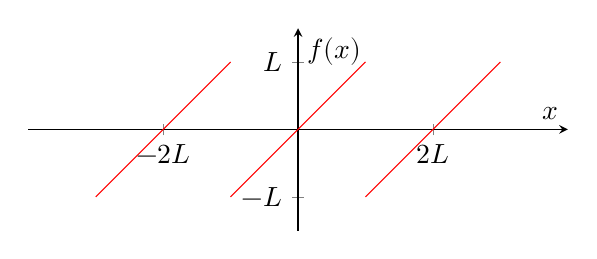
\begin{tikzpicture}
        \begin{axis}[
          xtick={-4,4},
          xticklabels={$-2L$,$2L$},
          ytick={-2,2},
          yticklabels={$-L$,$L$},
          axis lines=center,
          axis equal image,
          xmin=-8,
          xmax=8,
          ymin=-3,
          ymax=3,
          xlabel=$x$,
          ylabel=$f(x)$]
          \addplot[domain=-2:2,color=red]{x};
          \addplot[domain=2:6,color=red]{x-4};
          \addplot[domain=-6:-2,color=red]{x+4};
        \end{axis}
      \end{tikzpicture}
    \end{center}
    The function is odd so
\begin{align*}
  a_m &= \frac{1}{L}\int_{-L}^L x \cos\frac{m\pi x}{L} dx = 0 \\ 
  b_m  &= \frac{1}{L}\int_{-L}^L x \sin\frac{m\pi x}{L} dx \\
      &= \frac{1}{L}\Big[x \frac{L}{m\pi}(-\cos\frac{m\pi x}{L})\Big]_{-L}^L - \frac{1}{L}\frac{L}{m\pi} \int_{-L}^L -\cos\frac{m\pi x}{L} dx \\
      &= \frac{1}{m\pi}\Big( L(-\cos m\pi) - (-L)(-\cos m\pi) \Big) + \frac{1}{m\pi} \Big[ \frac{L}{m\pi} \sin\frac{m\pi x}{L} \Big]_{-L}^L \\
  &= \frac{2L}{m\pi}(-1)^{m+1}
\end{align*}

So
\[
  \frac{f(x_+)+f(x_-)}{2} = \frac{2L}{\pi}\Big[\sin\frac{\pi x}{L} - \frac{1}{2}\sin\frac{2\pi x}{L} + \cdots \Big].
\]
and we observe that
\begin{enumerate}
\item $f_N(x) = \sum_{n=1}^N b_n\sin\frac{n\pi x}{L} \to f(x)$ almost everywhere but the convergence is \emph{not} uniform.
\item Persistent overshooting at $x=L$: Gibbs phenomenon.
\item $f(L) = 0$, the average of right and left hand limit.
\item Coefficients are $O(\frac{1}{n})$ as $n\to \infty$.
\end{enumerate}

\item The integral of the sawtooth function, $f(x) = \frac{x^2}{2}$ for $-L \leq x < L$.
    \begin{center}
      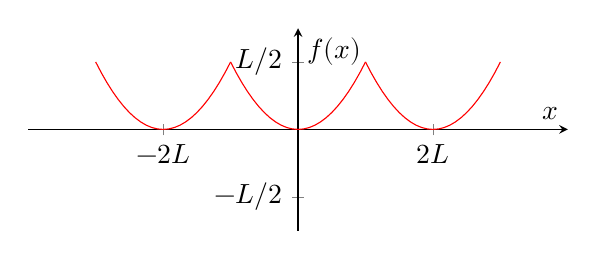
\begin{tikzpicture}
        \begin{axis}[
          xtick={-4,4},
          xticklabels={$-2L$,$2L$},
          ytick={-2,2},
          yticklabels={$-L/2$,$L/2$},
          axis lines=center,
          axis equal image,
          xmin=-8,
          xmax=8,
          ymin=-3,
          ymax=3,
          xlabel=$x$,
          ylabel=$f(x)$]
          \addplot[domain=-2:2,color=red]{x^2/2};
          \addplot[domain=2:6,color=red]{(x-4)^2/2};
          \addplot[domain=-6:-2,color=red]{(x+4)^2/2};
        \end{axis}
      \end{tikzpicture}
    \end{center}
  Exercise: $f(x) = L^2 \big[ \frac{1}{6} + 2\sum_{n=1}^\infty \frac{(-1)^n}{(n\pi)^2} \cos\frac{n\pi x}{L} \big]$.

  Note at $x=0$,
  \begin{align*}
    & 0 = L^2 \Big[\frac{1}{6} + 2\sum_{n=1}^\infty \frac{(-1)^n}{(n\pi)^2} \Big] \\
    \Rightarrow & \frac{\pi^2}{12} = \sum_{n=1}^\infty\frac{(-1)^{n+1}}{n^2}
  \end{align*}
  \end{enumerate}
\end{eg}

\section{Properties of Fourier Series}

\subsection{Integration \& Differentiation}

\subsubsection{Integration\protect\footnote{Don't panic: it's always OK.}}

Fourier series \emph{can} be integrated term by term. Suppose $f(x)$ with period $2L$ has a Fourier series (so it satisfies the Direichlet condition):
\[
  \frac{f(x_+)+f(x_-)}{2} = \frac{1}{2}a_0 + \sum_{n=1}^\infty \Big(a_n\cos\frac{n\pi x}{L} +b_n\sin\frac{n\pi x}{L}\Big).
\]
Consider
\begin{align*}
  F(x) & = \int_{-L}^x f(u) du \\
       &= \frac{a_0(x+L)}{2} + \sum_{n=1}^\infty \frac{a_n L}{n\pi}\sin\frac{n\pi x}{L} + \sum_{n=1}^\infty \frac{b_n L}{n\pi} \Big[(-1)^n - \cos\frac{n\pi x}{L} \Big] \\
       &= \frac{a_0 L}{2} + L \sum_{n=1}^\infty (-1)^n \frac{b_n}{n\pi} - L \sum_{n=1}^\infty \frac{b_n}{n\pi} \cos\frac{n\pi x}{L} \\
       &+ L \sum_{n=1}^\infty \frac{a_n-(-1)^n a_0}{n\pi}\sin\frac{n\pi x}{L}
\end{align*}

If $a_n, b_n$ are Fourier coefficients, then series involving $\frac{a_n}{n}, \frac{b_n}{n}$ (multiplied by sine or cosine) must also converge, so they are part of a Fourier series. Fourier series of $f(x)$ exists so $b_n$ is at least of $O(\frac{1}{n})$ as $n\to\infty$. Thus $\frac{b_n}{n}$ is at least of order $O(\frac{1}{n^2})$ as $n\to \infty$ and so by comparison test with $\sum \frac{M}{n^2}$ the second term converges, so $F(x)$ has a Fourier series.

\begin{note}
  Integration smoothes.
  The proof relies on discontinuity being bounded ($f(x)$ satisfies the Dirichlet condition).
\end{note}

\subsubsection{Differentiation\protect\footnote{Do panic, it doesn't always work!}}

Let $f(x)$ be a periodic function with period $2$ such that
\[
  f(x) =
  \begin{cases}
    1 & 0 < x < 1\\
    -1 & -1 < x < 0 
  \end{cases}
\]
This is an odd function so
\begin{align*}
  a_m &= 0 \\
  b_m &= -\int_{-1}^0 \sin m\pi x dx + \int_{-1}^0 \sin m\pi x dx \\
  &= \frac{\cos m\pi x}{m\pi} \Big|_{-1}^0 - \frac{\cos m\pi x}{m\pi} \Big|_0^{-1} \\
  &= \frac{1}{m\pi} \big(1- (-1)^m - (-1)^m + 1 \big) \\
  & =
  \begin{cases}
    \frac{4}{m\pi} & m \text{ is odd} \\
    0 & m \text{ is even}
  \end{cases}
\end{align*}
Thus
\[
  \frac{f(x_+)+f(x_-)}{2} = \frac{4}{\pi} \sum_{n=1}^\infty \frac{\sin(2n-1)\pi x}{2n-1}.
  \]
Apply differentiation rules
\[
  f'(x) = 4 \sum_{n=1}^\infty \cos(2n-1)\pi x
\]
This is clearly divergent even though $f'(x) = 0$ for all $x \neq 0$. The extra factor of $2n-1$ is the problem, which is related to the discontinuity. $f'(x)$ \emph{does not} satisfy the Dirichlet condition.

\begin{note}
  Intuitively, this behaviour can be explained by noticing that Dirac delta function is the derivative of Heaviside function.
\end{note}

\subsubsection{Differentiation Under Certain Circumstances}

Fourier series can be differentiated under certain circumstances: 
\begin{eg}
  Assume \(f(x)\) is continuous and is extended as a \(2L\)-periodic function, piecewise continuously differentiable on \((-L,L)\). Let \(g(x)=\frac{df}{dx}\). \(g(x)\) satisfies the Dirichlet condition as it has at worst a finite number of bounded discontinuities.
  \begin{align*}
    f(x) &= \frac{a_0}{2} + \sum_{n=1}^{\infty} a_n \cos \frac{n\pi x}{L}+ b_n \sin \frac{n\pi x}{L} \\
    \frac{g(x_+)+g(x_-)}{2} &=\frac{A_0}{2} + \sum_{n=1}^{\infty} A_n \cos \frac{n\pi x}{L} + B_n \sin \frac{n\pi x}{L}
  \end{align*}
  Then
  \begin{align*}
    A_0 &= \frac{1}{L}\int_{0}^{2L}g(x) dx \\
        &= \frac{f(2L)-f(0)}{L} \\
        &= 0
  \end{align*}
  by periodicity.
  \begin{align*}
    A_n &=\frac{1}{L} \int_{0}^{2L}\frac{df}{dx}\cos \frac{n\pi x}{L}dx \\
        &= \frac{1}{L}\Big[f(x)\cos \frac{n\pi x}{L} \Big] \Big|_0^{2L} + \frac{n\pi}{L^2} \int_{0}^{2L} f(x)\sin \frac{n\pi x}{L} dx \\
        &= 0 + \frac{n\pi b_n}{L}
      \end{align*}
      Similarly, \(B_n=-\frac{n\pi a_n}{L}\).

      This reduces differentiation to multiplication by \(\pm \frac{n\pi}{L}\).
      \end{eg}

\subsection{Alternate Representation: Complex Form}

Recall
\begin{align*}
  \cos \frac{n\pi x }{L} &= \frac{1}{2} (e^{i\frac{n\pi x}{L}} + e^{-i\frac{n\pi x}{L}}) \\
  \sin \frac{n\pi x }{L} &= \frac{1}{2i} (e^{i\frac{n\pi x}{L}} - e^{-i\frac{n\pi x}{L}})
\end{align*}
so
\begin{align*}
  \frac{f(x_+)+f(x_-)}{2} &= \frac{a_0}{2} + \sum_{n=1}^{\infty} \frac{a_n}{2} (e^{i \frac{n\pi x}{L}} + e^{-i \frac{n \pi x}{L}}) - \sum_{n=1}^{\infty} \frac{b_n}{2} (e^{i \frac{n\pi x}{L}} - e^{-i \frac{n \pi x}{L}})\\
                          &= \frac{a_0}{2} + \sum_{n=1}^{\infty} \big( \frac{a_n-i b_n}{2} e^{i \frac{n\pi x}{L}} \big) + \sum_{n=1}^{\infty} \big( \frac{a_n+i b_n}{2} e^{-i \frac{n\pi x}{L}} \big) \\
                          &= \sum_{n=-\infty}^{\infty} c_n e^{i\frac{n\pi x}{L}}
\end{align*}
with
\begin{align*}
  c_0 &= \frac{a_0}{2}, \\
  c_n &= \frac{a_n-ib_n}{2}, n>0, \\
  c_n &= \frac{a_n+ib_n}{2}, n<0.
\end{align*}

Note that \(c_n^* = c_{-n}\). It can be easily shown that complex exponentials are orthogonal:
\begin{align*}
  \int_{0}^{2L} e^{i\frac{n\pi x}{L}} e^{-i\frac{m\pi x}{L}}dx &= \int_{0}^{2L}\cos \frac{(n-m)\pi x}{L}dx + i \int_{0 }^{2L}\sin \frac{(n-m)\pi x}{L} dx \\
  &= 2L \delta_{n,m} + 0
\end{align*}
so
\[
  c_m = \frac{1}{2L} \int_{0}^{2L}f(x)e^{-i\frac{m\pi x}{L}} dx = \frac{1}{2L} \int_{0}^{2L} \Big( \sum_{n=-\infty}^{\infty} c_n e^{i\frac{n\pi x}{L}} \Big) e^{i\frac{-m\pi x}{L}} dx.
\]

Now assume \(g(x) = \frac{df}{dx} = \sum_{n=-\infty}^{\infty} c_n e^{i\frac{n\pi x}{L}}\). Then
\begin{align*}
  c_n &= \frac{1}{2L}\int_{0}^{2L} \frac{df}{dx }e^{-i\frac{n\pi x}{L}}dx \\
      &= \frac{1}{2L} \Big[ f(x) e^{-i\frac{n\pi x}{L}} \Big]_0^{2L} + \frac{in\pi}{2L^2} \int_{0}^{2L}f(x) e^{-i\frac{n\pi x}{L}} dx \\
      &= \frac{in\pi}{L}c_n
\end{align*}
by periodicity.



\subsection{Half-range Series}

Consider a function defined \emph{only} on \(0 \leq x \leq L\). There are two possible ways to extend this function to a \(2L\)-periodic function that can be represented as a Fourier series.

\subsubsection{Odd function: Fourier Sine Series}

\(f(x)\) can be extended as an \emph{odd} function \(f(x)=-f(-x)\) on \(-L \leq x \leq L\) and then extended as a \(2L\)-periodic function. In this case \(a_n=0\) we can define the \emph{Fourier sine series}:
\[
  \frac{f(x_+)+f(x_-)}{2} = \sum_{n=1}^{\infty}b_n \sin \frac{n\pi x}{L}
\]
where
\[
  b_n = \frac{2}{L} \int_{0}^{L} f(x) \sin \frac{n\pi x}{L} dx.
\]
Note the range of integration.

\begin{eg}[Sawtooth function]
  
\end{eg}

\subsubsection{Even function: Fourier Cosine Series}

\(f(x)\) can also be extended as an even function on \(-L\leq x\leq L\), i.e.\ \(f(x) = f(-x)\) and then extended as a \(2L\)-periodic function. \(b_n=0\) for all \(n\). The Fourier cosine series is
\[
  \frac{f(x)+f(x)}{2} = \frac{a_0}{2} + \sum_{n-1}^{\infty}a_n \cos \frac{n\pi x}{L}
\]
where
\[
  a_n = \frac{2}{L}\int_{0}^{L}f(x)\cos \frac{n\pi x}{L}.
\]

\subsection{Parseval's Theorem}

``Energy'' of a periodic signal is often of interest, i.e.\ \(E = \int_{0}^{2L}f^2(x) dx \). Consider the general case
\[
  f(x) = \sum_{n=-\infty}^{\infty}c_n e^{\frac{in\pi x}{L}}, g(x) = \sum_{m=-\infty}^{\infty}d_m e^{\frac{im\pi x}{L}};
\]
\begin{align*}
  \int_{0}^{2L} f(x) g(x) dx &= \sum_{n=-\infty}^{\infty} \sum_{m=-\infty}^{\infty} c_n d_m \int_{0}^{2L} \exp \Big [\frac{i\pi x}{L} (n+m) \Big] dx \\
  &= \sum_{n=-\infty}^{\infty} \sum_{m=\infty}^{\infty} c_n d_m (2L \delta_{n,-m}) \\
  &= 2L \sum_{n=-\infty}^{\infty} c_n d_{-n} \\
  &= 2L \sum_{n=-\infty}^{\infty} c_n d_n^*
  \end{align*}
so if \(g=f\),
\[
  \int_{0}^{2L} f^2(x) dx = 2L \sum_{n=-\infty}^{\infty}|c_n|^2 = L \Big[ \frac{a_0^2}{2} + \sum_{n=1}^{\infty}(a_n^2+b_n^2) \Big]
\]

\begin{eg}[Sawtooth function]
  Remember \(f(x)=x\) for \(-L\leq x\leq L\).
  \[
    b_n = \frac{2L}{m\pi}(-1)^{m+1}
  \]
  so
  \[
    \int_{-L}^{L} x^2 dx = \frac{2L^3}{3} = L \sum_{m=1}^{\infty}\frac{4L^2}{m^2\pi^2}
  \]
  so
  \[
    \sum_{m=1}^{\infty}\frac{1}{m^2} = \frac{\pi^2}{6}.
  \]
\end{eg}

\begin{ex}
  From the Fourier series of \(x^2/2\) show that
  \[
    \sum_{m=1}^{\infty}\frac{1}{m^4} = \frac{\pi^4}{90}.
  \]
\end{ex}

\section{Sturm-Liouville Theory}

\subsection{Second Order ODEs}

Consider a general second order ordinary partical differential equation
\[
  \L y(x) = \alpha(x) \frac{d^2y}{dx^2} + \beta(x) \frac{dy}{dx} + \gamma(x) y = f(x).
\]

\(\alpha,\beta,\gamma\) are continuous, with \(\alpha\) non-zero except perhaps at a finite number of isolated points. \(f(x)\) is bounded, defined on \(a\leq x\leq b\) (\(a\) or \(b\) may be infinity).
tary function is \[
  y_c=Ay_1+By_2.
\]
\emph{Inhomogeneous} or \emph{forced} equation \(\L y = f(x)\) where \(f\) is the forcing, has a particular integral \(y_p(x)\). The general solution is \(y=y_c(x)+y_p(x)\) where \(A,B\) are determined in a problem by applying condition.

\subsection{Hermitian Matrices: an Analogy}

Remember the problem: find \(\V x \) such that
\[
A \V x = \V b.
\]
If \(A\) is an Hermitian matrix, \(A\) is \(N \times N\), i.e.\ \(A^\dag A\) where the \(\dag\) denotes complex conjugate transpose. It has \(4\) properties:\footnote{Recall an eigenvector and eigenvalue are defined such that \(A \V y_n = \lambda_n \V y_n\) where \(\lambda_n\) is the eigenvalue and \(y_n\) is the eigenvector.}
\begin{enumerate}
\item \(\lambda_n\) are real,
\item if \(\lambda_m\neq\lambda_n\) then \(\V y_m\cdot\V y_n=0\),
\item the eigenvectors form, on scaling, an orthonormal basis and so specially \(\V b \in \C^N\) can be described by a linear combination of eigenvectors,
\item if \(A\) is non-singular, i.e.\ all eigenvalues are non-zero, the solution to \(A\V x = \V b\) can be written as a sum of eigenvector.
\end{enumerate}

\subsubsection{Gaussian Elimination}

From property \(3\) above we can write
\begin{align*}
  \V b &= \sum_{n=1}^{N}b_n y_n \\
  \V x &=\sum_{n=1}^{N}C_n y_n
\end{align*}

Since \(A\) is linear,
\[
  A \V x = \sum_{n=1}^{N}c_n A \V y_n = \sum_{n=1}^{N}c_n \lambda_n \V y_n = \sum_{n=1}^{N}b_n \V y_n = \V b.
\]
For simplicity assuming the \(\lambda_n\) are distinct and non-zero. From property \(2\),
\[
\V y_m \cdot \big( \sum_{n=1}^{N}c_n \lambda_n \V y_n \big) = c_m \lambda_m = \V y_m \cdot \big( \sum_{n=1}^{N}c_n \lambda_n \V y_n \big) = b_m
\]
Therefore
\begin{align*}
  c_m &= \frac{b_m}{\lambda_m} \\
  x &= \sum_{n=1}^{N}\frac{b_n}{\lambda_n}y_n
\end{align*}

\begin{question}
  Can this be generalised to differential operators?
\end{question}

\subsection{Motivating Example: Fourier Series}
\label{subsec:motivating}

For continuous forcing functions \(f(x)\), we want to find \(y(x)\) on a finite interval such that
\[
  -\frac{d^2y}{dx^2} = f(x), 0 \leq x \leq L, \: f(0) = f(L) = y(0) = y(L) = 0,
\]
satisfies the Dirichlet conditions and so we can write a Fourier sine series if we extend \(f\) to be a \(2L\)-periodic odd function:
\begin{align*}
  f(x) &= \sum_{n=1}^{\infty}b_n \sin \frac{n\pi x}{L} \\
  b_n &= \frac{2}{L} \int_{0}^{L} f(\xi) \sin \frac{n\pi \xi}{L} d\xi
\end{align*}

Let \(\L = - \frac{d^2}{dx^2}\), can we find solutions to
\[
\L y_n = \lambda_n y_n,\: y_n(0) = y_n(L) = 0?
\]

Indeed, we can solve the equations
\[
  \frac{d^2}{dx^2} y_n = - \lambda_n y_n,
\]
and obtain the solutions
\begin{align*}
  y_n &= \sin \frac{n\pi x}{L}, \\
  \lambda_n &= \frac{n^2\pi^2}{L^2}.
\end{align*}
In particular, the boundary value quantises the \(\lambda_n\).

\begin{note}
  \(\lambda_n\) are real and strictly positive and so \(y_n\) is an eigenfunction with associated eigenvalue \(\lambda_n\).
\end{note}

Note \(\lambda_n = \frac{n^2\pi^2}{L^2}\) has property \(1\) and we have already met the orthogonality property \(2\), i.e.\ \(\int_{0}^{L} y_ny_m dx=\frac{L}{2}\delta_{m,n} \). There is also a generalisation of property \(3\): sines and cosines form a complete (infinite-dimensional) basis for functions that satisfy Dirichlet condition.

For this problem \(y(x)\) must be sufficiently smooth so that its \emph{second derivative} satisfies the Dirichlet condition.

\(y(x)\) has a Fourier sine series:
\begin{align*}
  y(x) &= \sum_{n=1}^{\infty}c_n \sin \frac{n\pi x}{L} \\
  -\frac{d^2}{dx^2} y &= \L y = \sum_{n=1}^{\infty} \frac{n^2\pi^2}{L^2}c_n \sin \frac{n\pi x}{L} = \sum_{n=1}^{\infty} \lambda_n c_n \sin \frac{n\pi x}{L} \\
       &= \sum_{n=1}^{\infty}b_n \sin \frac{n\pi x}{L}
\end{align*}

The orthogonality property tell us that
\[
\lambda_n c_n = b_n.
\]
Thus
\begin{align*}
  y(x) &= \sum_{n=1}^{\infty} \frac{b_n}{\lambda_n} \sin \frac{n\pi x}{L}, \: \lambda_n = \frac{n^2\pi^2}{L^2} \\
       &= \frac{2}{L} \int_{0}^{L} \sum_{n=1}^{\infty} \frac{1}{\lambda_n} \sin \frac{n\pi x}{L}\sin\frac{n\pi\xi}{L} f(\xi) d\xi \\
        &= \int_{0}^{L} G(x; \xi) f(\xi) d\xi\end{align*}
where \(G(x;\xi)\) is the \emph{Green's function}.

Note the loose analogy between Hermitian matrices and self-adjoint operators:
\begin{align*}
  A\V x = \V b &\Rightarrow \V x = A^{-1}\V b \\
  \L y = f &\Rightarrow y = \L^{-1} f
\end{align*}

\section{Self-adjoint Operators}

\subsection{Definition of Self-adjoint Form}

Consider a second order linear differential operator where the eigenvalue problem is to determine eigenfunction \(y\) and associated eigenvalue \(\lambda\) such that
\begin{equation}
  \label{eqn:self-adjoint}
\alpha(x) \frac{d^2y}{dx^2} + \beta(x) \frac{dy}{dx} + \gamma(x) y = \L y = -\lambda \kappa(x) y, a \leq x\leq b
\tag{\(\ast\)}
\end{equation}
where \(\kappa\) and \(\alpha\) are real and positive on \([a,b]\). (In the previous example, \(\kappa = 1 = \alpha, \beta=\gamma=0\).) This general differential operator can \emph{always} be written in \emph{Sturm-Liouville} or \emph{self-adjoint} form
\[
\L y = - \frac{d}{dx} \Big[ p(x) \frac{dy}{dx} \Big] + q(x) y =\lambda w(x) y
\]
where \(w(x)\) is called the \emph{weight} function, wlog real and positive on \([a,b]\) except possibly on isolated points where \(w=0\).

Multiply \eqref{eqn:self-adjoint} by \(-\phi(x)\) where
\[
\phi(x) = \frac{1}{\alpha(x)}\exp \Big(\int_{ }^{x} \frac{\beta(u)}{\alpha(u)} du \Big),
\]
the result is
\begin{align*}
  p(x) &= \exp \Big( \int^x \frac{\beta(u)}{\alpha(u)}du \Big) \\
  q(x) &= -\frac{\gamma(x)}{\alpha(x)} \Big( \int^x \frac{\beta(u)}{\alpha(u)}du \Big) \\
  w(x) &= -\frac{\kappa(x)}{\alpha(x)} \Big( \int^x \frac{\beta(u)}{\alpha(u)}du \Big)
\end{align*}
where \(p, q, w\) are all real and positive on \([a,b]\).

\subsection{Definition of Self-adjointness}

Consider a linear \(2\)nd order differential operator \(\L\) defined on \([a,b]\). The \emph{adjoint} of \(\L\), denoted by \(\L^\dag\) has the property that for all pairs of functions \(y_1\) and \(y_2\) satisfying appropriate boundary conditions, which shall be defined below,
\[
\int_a^b y_1^* \L y_2 dx = \int_a^b y_2 (\L^\dag y_1)^* dx.
\]
If \(\L = \L^\dag\) (with appropriate boundary conditions) then \(\L\) is said to be \emph{self-adjoint} or \emph{Hermitian}.

\subsubsection{Self-adjointness of Sturm-Liouville Operator}

To derive the necessary and sufficient condition for the Sturm-Liouville operator to be self-adjoint, we consider the real case here:
\begin{align*}
  \int_{a}^{b} y_1\L y_2 dx &= \int_{a}^{b} y_1 \Big[ -\frac{d}{dx} \big(p \frac{dy_2}{dx} \big) + qy_2 \Big] dx \\
                         &= \Big[-y_1 p\frac{dy_2}{dx} \Big]^b_a + \int_{a}^{b} qy_1y_2  dx + \int_{a}^{b} p\frac{dy_2}{dx} \frac{dy_1}{dx} dx \\
                         &= \Big[-y_1p \frac{dy_2}{dx} \Big]^b_a + \int_{a}^{b} y_2\Big(-\frac{d}{dx} \big(p \frac{dy_1}{dx} \big)+ qy_1 \Big) dx + \Big[ y_2p \frac{dy_1}{dx} \Big]^b_a \\
                         &= \int_{a}^{b} y_2\L y_1 dx + \underbrace{\Big[ p(y_2 \frac{dy_1}{dx} - y_1 \frac{dy_2}{dx})\Big]^b_a}_{T_1} 
\end{align*}
Note the Wronskian in \(T_1\).

The operator
\[
  \L = -\frac{d}{dx}(p \frac{d}{dx}) + q
\]
is thus self-adjoint if and only if \(T_1=0\).

In the previous example, \(y=0\) at \(x=a,b\). Other simple examples satisfying \(T_1=0\) include:
\begin{itemize}
\item \(y'=0\) at \(x=a,b\),
\item \(y+ky'=0\) with \(k\) constant at \(x=a,b\).
\item Periodic boundary conditions satisfying
\[
y(a) = y(b) \text{ or } y'(a) = y'(b).
\]
\item \(p=0\) at \(x=a,b\).
\end{itemize}

\subsubsection{Properties of Self-adjoint Operators}

\begin{enumerate}
\item The eigenvalues are real: assume that \(\lambda_n\) is an eigenvalue and \(y_n\) is the associated eigenfunction. Then
  \[
\L y_n = \lambda_ny_n w, \: (\L y_n)^* = \lambda_n^*y_n^*w^*.
  \]
  But here \(w\) and \(\L\) are real by assumption (unlike in quantum mechanics, for example) so
  \begin{align*}
    \L y_n^* &= \lambda_n^* y_n^* w \\
    \int_{a}^{b} y_n(\L y_n^*) dx &=  \int_{a}^{b} y_n(\lambda_n^*wy_n^*) dx = \lambda_n^* \int_{a}^{b} w |y_n|^2 dx \\
    \int_{a}^{b} y_n^* (\L y_n) dx &= \int_{a}^{b} y_n^*(\lambda_ny_nw) dx = \lambda_n \int_{a}^{b} w |y_n|^2 dx
  \end{align*}
  By self-adjointness,
  \begin{align*}
    0 &= \int_{a}^{b} y_n (\L y_n)^* dx - \int_{a}^{b} y_n^* (\L y_n) dx \\
      &= (\lambda_n^* - \lambda_n) \int_{ }^{ } w |y_n|^2 dx
  \end{align*}
  so \(\lambda_n^* = \lambda_n\).
\item The eigenfunctions of distinct eigenvalues are orthogonal: assume that \(y_n\) and \(y_m\) are eigenfunctions with distinct eigenvalues \(\lambda_n \neq \lambda_m\):
  \[
\L y_n = \lambda_n w y_n, \: \L y_m = \lambda_m wy_m.
\]
By self-adjointness
\begin{align*}
  0 &= \int_{a}^{b} y_m\L y_n dx - \int_{a}^{b} y_n\L y_m dx \\
    &= \int_{a}^{b} y_m \lambda_nwy_n dx - \int_{a}^{b} y_n\lambda_mwy_m dx \\
    &= (\lambda_n - \lambda_m) \int_{a}^{b} wy_ny_m dx \\
  \Rightarrow &\int_{a}^{b} wy_ny_m dx = 0
\end{align*}

Note the weight function in the integral.
\item There is an orthonormal set of eigenfunctions: let
  \[
    Y_n(x) = \frac{y_n(x)}{\big(\int_{a}^{b} wy_n^2 dx \big)^{1/2}}
  \]
  so
  \[
\delta_{m,n}=\int_{a}^{b} w(x)Y_m(x)Y_n(x) dx.
  \]
\item The set of eigenfunctions form a complete basis: suppose a function \(f(x)\) satisfying the boundary condition as eigenfunction. \emph{Completeness} means that any such \(f(x)\) can be expressed as
  \[
f(x) = \sum_{n=1}^{\infty}a_ny_n(x) = \sum_{n=1}^{\infty} A_n Y_n(x).
  \]
  where \(Y_n(x)\) is an orthonormal basis.
\item These coefficients can always be determined using orthogonality:
  \[
\int_{a}^{b} f(x)wY_m(x) dx = \sum_{n=1}^{\infty}A_n \int_{a}^{b} wY_n(x)Y_m(x) dx = A_m
\]
\item A corollary of the property of completeness is that there is always a \emph{countably infinite} number of eigenvalues which satisfy the underlying self-adjoint problem.
\item Parseval's Theorem for such self-adjoint operators: consider
  \begin{align*}
    I &= \int_{a}^{b} w \underbrace{\Big[ f(x) - \sum_{n=1}^{\infty}A_nY_n(x) \Big]^2} dx \\
      &= \int_{a}^{b} w f^2(x) dx - 2 \sum_{n=1}^{\infty}A_n \int_{a}^{b} w fY_n dx + \sum_{n=1}^{\infty}\sum_{m=1}^{\infty} A_nA_m \int_{a}^{b} wY_nY_m dx \\
      &=\int_{a}^{b} w f^2 dx -2 \sum_{n=1}^{\infty}A_n^2 + \sum_{n=1}^{\infty}A_n^2 \\
      &= \int_{a}^{b} wf^2 dx - \sum_{n=1}^{\infty} A_n^2
  \end{align*}
  \begin{itemize}
  \item If the eigenfunctions are complete, \(I=0\) and so there is a Parseval's relation
  \[
\int_{a}^{b} wf^2 dx = \sum_{n=1}^{\infty}A_n^2.
  \]
\item If the eigenfunctions are not complete, e.g. if \(\L\) is \emph{not} self-adjoint, then square bracket term is positive, \(w\) is positive by construction. Therefore we get \emph{Bessel's inequaility}:
  \[
\int_{a}^{b} wf^2 dx \geq \sum_{n=1}^{\infty}A_n^2.
  \]
  \end{itemize}
\item Eigenfunction series representation are the ``best'' such representation in a particular sense: define the partial sum
  \[
    s_N(x) = \sum_{n=1}^{N}A_nY_n.
  \]
  Completeness implies that \(f(x) = \lim_{N\to \infty}s_N(x)\) except at points of discontinuity of \(f(x)\). For simplicity consider continuous \(f(x)\). The mean square error \(\varepsilon_N\) in approximating \(f(x)\) by \(s_N(x)\) is
  \[
\varepsilon_N = \int_{a}^{b} w(f-s_N(x))^2 dx \to 0 \text{ as } N\to \infty.
\]
Differentiate,
\begin{align*}
  \frac{\partial\varepsilon_n}{\partial A_m} &= -2 \int_{a}^{b} w \Big(f- \sum_{n=1}^{N}A_nY_n \Big) Y_m dx \\
                                             &= -2 \int_{a}^{b} wfY_m dx + 2 \sum_{n=1}^{N}A_n \int_{a}^{b} wY_nY_m dx \\
                                             &= -2A_m + 2A_m \\
                                             &= 0
\end{align*}
Therefore the coefficients extremise (in this case, minimise) the error in the mean square sense and so the best partial sum representation is the partial representation using the eigenfunctions of the underlying Sturm-Liouville operator.
  
\subsubsection{Example with Non-trivial Weight}

Problem: find \(y(x)\) on \([0,\pi]\) such that
\begin{align*}
  y'' + y' + (\frac{1}{4} + \lambda)y &=0 \\
  y(0) &= 0 \\
  y(\pi) - 2y'|_\pi &=0
\end{align*}

Write in self-adjoint form:
\[
  - \frac{d}{dx}\Big( e^x \frac{dy}{dx} \Big)- \frac{e^xy}{4} = \lambda e^xy.
\]
The auxillary equation \(y \propto e^{\sigma x}\) is
\[
  \sigma^2 + \sigma + \frac{1}{4} + \lambda = 0
\]
so
\[
  \sigma = -\frac{1}{2} \pm i \sqrt{\lambda}.
\]
The homogeneous solution is
\[
  y(x) = A e^{-x/2}\cos\mu x + B e^{-x/2}\sin\mu x
\]
with \(\mu^2=\lambda\), satisfying
\begin{align*}
  y(0) &= 0, \\
  y(\pi) - 2y'(\pi) &= Be^{-\pi/2}\big( \sin\mu\pi + \sin\mu\pi - 2\mu\cos\mu\pi \big)=0.
\end{align*}
Therefore
\begin{align*}
  A &= 0, \\
  \tan\mu\pi &= \mu.
\end{align*}
A simple plot shows that there are countably infinite eigenvalues that satisfy this equation. As \(n\to \infty,\mu_n \approx \frac{2n+1}{2}\).

Notice that the eigenfucntions are proportional to \(e^{-x/2}\sin\mu_nx\) so
\begin{align*}
  I_{mn} &\propto \alpha\int_{0}^{\pi} wy_n(x)y_m(x) dx \\
         &= \int_{0}^{\pi} e^x e^{-x/2}\sin\mu_nx e^{-x/2}\sin\mu_mx dx \\
         &= \int_{0}^{\pi} \sin\mu_nx \sin\mu_mx dx \\
         &= 0 \text{ if } n \neq m
\end{align*}
\end{enumerate}

\subsubsection{Application in Inhomogeneous Boundary Value Problems}

Consider this inhomogeneous problem:
\[
  (\L - \hat \lambda w)y = f(x) = wF(x) = w(x) \sum_{n=0}^{\infty} A_nY_n(x).
\]
By completeness, \(y = \sum_{n=1}^{\infty} B_nY_n(x) \) where \(B_n\) is the unknown.
\begin{align*}
  w \sum_{n=1}^{\infty}A_nY_n &= \sum_{n=1}^{\infty}B_n (\L Y_n - \hat \lambda w Y_n) \\
  &= \sum_{n=1}^{\infty}B_n(\lambda_n-\hat \lambda)wY_n
\end{align*}
Multiply across by \(Y_m\) and use property 4: \(\delta_{mn} = \int_{a}^{b} wY_nY_m dx \):
\[
  A_m = B_m(\lambda_m-\hat \lambda)
\]
so
\begin{align*}
  B_m &= \frac{A_m}{\lambda_m-\hat\lambda} \\
      &= \frac{\int_{a}^{b} w(\xi)Y_m(\xi)F(\xi) d\xi}{\lambda_m-\hat\lambda} \\
      &= \frac{\int_{a}^{b} Y_m(\xi)f(\xi) d\xi}{\lambda_m-\hat\lambda} \\ 
  y(x) &= \int_{a}^{b}  \sum_{n=1}^{\infty} \frac{Y_n(\xi)Y_n(x)}{\lambda_n-\hat \lambda} f(\xi) d\xi \\
      &= \int_{a}^{b} G(x;\xi)f(\xi) d\xi
\end{align*}
which is the general form of the example in section~\ref{subsec:motivating}.

% Part II: Seperation of Variables

\section{Wave Equation}

Wave equation is a canonical second order PDE: an example of \emph{hyperbolic equation}. Whenever you have a system with low dissipation of energy and a restoring force you have a wave.

The linear wave equation takes the form
\[
\frac{\p^2\phi}{\p t^2} = c^2\nabla^2\phi
\]
where \(c\) is the (phase) speed, i.e.\ speed of propagation of crests.

\subsection{Physical Derivation}

The simplest example is a heavy ``massive'' elastic string suspended between \(x=0\) and \(x=L\). Assume those points are at \(y=0\) and assume all deflections are sufficiently small that we can consider them to be vertical. Therefore \(y(x,t)\) describes the deflections.

Tension \(T(x)\) in the string, restoring forces horizontally and vertically:

The horizontal forces satisfy
\[
  T(x)\cos\theta_1 = T(x+\delta x)\cos\theta_2,\, |\theta_1|,|\theta_2| \ll 1,
\]
so
\[
T(\theta) \approx T(x+\delta x)
\]
so \(T\) is a constant.

We further assume that there is no horizontal motion and the mass of string per unit length is \(\mu\). The vertical force
\[
\mu\delta x \frac{\p^2 y}{\p t^2} = T\sin \theta_2 -T\sin\theta_1 - \mu g\delta x
\]
For small angles,
\begin{align*}
  \sin \theta_2 &\approx \tan\theta_2 = \frac{\p y}{\p x}\Big|_{x+\delta x} \approx \frac{\p y}{\p x}\Big|x + \delta x \frac{\p^2 y}{\p x^2}\Big|x \\
  \sin \theta_1 &\approx \tan\theta_1 = \frac{\p y}{\p x}\Big|_x
\end{align*}
so
\[
  \mu\delta x \frac{\p^2 y}{\p x^2} = T\delta x \frac{\p^2 y}{\p x^2} - \mu g\delta x + O(\delta x^2).
\]
We now assume that the weight of the string plays no role:
\[
  g\to 0 \text{ or } \frac{T\p^2 y}{\mu\p x^2} \gg g
\]
so
\[
  \frac{\p^2 y}{\p x^2} = \frac{T}{\mu} \frac{\p^2 y}{\p x^2} = c^2\frac{\p^2 y}{\p x^2}
\]

\subsection{Example: Wave on a Finite String}

We want to  find the displacement \(y(x,t)\) such that
\begin{align*}
  \frac{\p^2 y}{\p x^2} &= c^2 \frac{\p^2 y}{\p x^2} \\
  y(0,t) &= y(L,t) = 0 \\
  y(x,0) &= \phi(x) \\
  \frac{\p y(x,0)}{\p x} &= \psi(x)
\end{align*}

We use \emph{seperation of variables}. At its heart there is an existence and uniqueness proof. If we can find a solution by \emph{any means} it is the unique solution.

Suppose
\[
y(x,t) = X(x)T(t),
\]
substitute
\begin{align*}
  X \ddot{T} &= c^2X''T \\
  \frac{1}{c^2} \frac{\ddot{T}}{T} &= \frac{X''}{X} = -\lambda
\end{align*}
so we have two equations:
\begin{align*}
  X'' &= -\lambda X \\
  \ddot{T} &= -\lambda c^2 Y \\
  X(0) &= 0 \\
  X(L) &= L
\end{align*}
\(\lambda\geq0\) as otherwise \(X\) has at most \(1\) zero. Solve \(X\) to get
\[
  X = \alpha \cos \sqrt\lambda x + \beta \sin\sqrt\lambda x \\
\]
so
\[
  \lambda_n = \frac{n^2\pi^2}{L^2}, \, n \in \N.
\]
Note that these are real eigenvalues of the Sturm-Liouville system
\[
  -\frac{d}{dx} \big(\frac{dX}{dx} \big) = \lambda X.
\]
The associated eigenfunctions are the \emph{normal modes}:
\[
  X_n(x) = \beta_n \sin \frac{n\pi x}{L}.
\]
The lowest mode, i.e.\ \(n=1\), is the \emph{fundamental mode} while \(n=2,3,\dots\) are the \emph{overtones}.

Note how the eigenvalues \emph{quantise} the admissible solutions. For each of the \(X_n\) there is an associated \(T_n(t)\):
\[
  \ddot{T}_n = -\frac{n^2\pi^2c^2}{L^2}T_n
\]
which has solution
\[
  T_n = \gamma_n \cos \frac{n\pi ct}{L} + \delta_n \sin \frac{n\pi ct}{L}.
\]
Combining the two parts,
\[
  y_n(x,t) = X_n(x)T_n(t) = \sin \frac{n\pi x}{L} \Big( A_n \cos \frac{n\pi ct}{L} + B_n \sin \frac{n\pi ct}{L} \Big).
\]

The wave equation is linear so we can add all these solutions together
\begin{align*}
  y(x,t) &= \sum_{n=1}^{\infty} \sin \frac{n\pi x}{L} \Big( A_n \cos \frac{n\pi ct}{L} + B_n \sin \frac{n\pi ct}{L} \Big) \\
         &= \sum_{n=1}^{\infty} b_n(t) \sin \frac{n\pi x}{L}
\end{align*}
which is naturally a Fourier sine series. The \(A_n\) and \(B_n\) are determined from initial conditions:
\begin{align*}
  &y(x,0) = \phi(x) = \sum_{n=1}^{\infty} A_n \sin \frac{n\pi x}{L} \\
  \Rightarrow & A_n = \frac{2}{L} \int_{0}^{L} \phi(x) \sin \frac{n\pi x}{L} dx \\
  & \frac{\p y(x,0)}{\p t} = \psi(x) = \sum_{n=1}^{\infty} \frac{n\pi cB_n}{L} \sin \frac{n\pi x}{L} \\
  \Rightarrow & B_n = \frac{2}{n\pi c} \int_{0}^{L} \psi(x) \sin \frac{n\pi x}{L} dx
\end{align*}

\subsection{Algorithm for Seperation of Variables}

The algorithm for seperation of variables is clear:
\begin{enumerate}
\item seperate the variables: write \(y(x,t)=X(x)T(t)\),
\item determine the admissable form for eigenvalues and associated eigenfunctions from boundary conditions (i.e.\ conditions on \(x\)),
\item determine the form of the other seperated function using the eigenvalues and find a particular set of solution \(y_n\),
\item sum over all \(y_n\) to form a series representation,
\item determine the coefficients from the initial condititions (i.e.\ conditions on \(t\)).
\end{enumerate}

\begin{ex}
  Determine the full solution for a plucked string
  \[
    \psi(x) =0, \phi(z) =
    \begin{cases}
      \phi_0\frac{x}{d} & 0 \leq x \leq d \\
      \phi_0\frac{L-x}{L-d} & d \leq x \leq L
    \end{cases}
  \]
\end{ex}

\section{Bessel's Equation}

\subsection{Derivation of Bessel's Equation}

\label{subsec:derivation of Bessel}

Consider the wave equation on the unit disc
\[
  \frac{\partial^2 u}{\partial t^2} = c^2 \frac{\partial^2 u}{\partial x^2} + c^2 \frac{\partial^2 u}{\partial y^2} = c^2\nabla^2u, \, x^2+y^2\leq 1
\]
As usual, use seperation of varaibles:
\begin{enumerate}%remove
\item \(u(x,y,t) = V(x,y)T(t)\), \(\ddot T = -\lambda c^2T, \nabla^2V = -\lambda V\) with \(\lambda \geq 0\), since we are in the unit disc,
  \[
    V(x,y) = R(r) \Theta(\theta)
  \]
  so
  \begin{align*}
    \frac{\partial^2 V}{\partial r^2} + \frac{1}{r^2} \frac{\partial^2 V}{\partial \theta^2} + \frac{1}{r}\frac{\partial V}{\partial r} + \lambda V &= 0 \\
    R''\Theta + \frac{1}{r^2} R\Theta'' + \frac{1}{r}R'\Theta+\lambda R\theta &= 0 \\
    r^2R''\Theta+rR'\Theta+\lambda r^2R\Theta &= -R\Theta''
  \end{align*}
  Divide by \(R\Theta\), we get
  \[
    f_2(r) = f_1(\theta) = \mu
  \]
  Due to circular gemoetry \(\Theta\) must be periodic with period \(2\pi\). Thus \(\mu = m^2\), where \(m\) is an integer. This implies that
  \[
    r^2R'' + rR' + (\lambda r^2-m^2)R = 0.
  \]
  Now dividing across by \(-r\) to put this in Sturm-Liouville form:
  \[
    -\frac{d}{dr}\big( r \frac{d R}{d r} \big) + \frac{m^2}{r}R = \lambda r R, \, r\leq 1
  \]
  which has non-trivial weigtht. Furthermore let \(z = \sqrt\lambda r\) this can be reposed as
  \[
    z^2 \frac{d^2 R}{dz^2} + z \frac{d R}{d z} + (z^2-m^2)R = 0.
  \]
  This is \emph{Bessel's equation}.
\end{enumerate}

Solution to this equation are called \emph{Bessel functions of the first kind and second kind}.

\subsection{Properties of Bessel Functions}

\begin{enumerate}
\item \(J_m(z)\), the Bessel function of the frist kind of order \(m\) which is regular at the origin (and is \(0\) there for \(m>0\)) \(m=0\) for axis symmetric solution (i.e.\ solutions independent of \(\Theta\)).
\item \(Y_m(z)\) the Bessel function of the second kind which are singular at the origin.\footnote{Note \(Y_m(z)\) here is \emph{not} orthonormal.} Sometimes called Neumann function \(N_m\) or Weber function.
\end{enumerate}
    
Some properities of the Bessel functions include:

\begin{itemize}
\item \(J_\nu(z)\) has a series expansion (\(\nu\) not an integer in general):
  \[
    J_\nu(z) = \Big( \frac{z}{2} \Big)^\nu \sum_{n=0}^{\infty} \frac{(-z^2/4)^k}{k!\Gamma(\nu+k+1)}
  \]
  where \(\Gamma\) is the Gamma function.

\item \(J_\nu\) and \(J_{-\nu}\) are linearly independent for non-integer \(\nu\).
\item \(Y_\nu(z)\) is defined by
  \[
    \frac{J_\nu(z)\cos\nu\pi - J_{-\nu}(z)}{\sin\nu\pi}.
  \]

\item For integer \(\nu=m\):
  \begin{align*}
    J_{-m}(z) &= (-1)^m J_m(z) \\
    Y_{-m}(z) &= (-1)^m Y_m(z) \\
    Y_m(z) &= \lim_{\nu\to m} \frac{J_\nu(z)\cos\nu\pi - J_{-\nu}}{\sin \nu\pi}.
  \end{align*}
\item \(Y_0(z) \approx \frac{2}{\pi} \log z, \, J_0\approx 1 \text{ as } z\to 0 \).
\item \(Y_m(z) \approx - \frac{1}{\pi} \Big( \frac{2}{\pi} \Big)^{-m} (m-1)!,\, J_m \approx \frac{(z/2)^m}{m!} \to 0\) for \(m>0\).
\item As \(z\to \infty\),
  \begin{align*}
    J_\nu(z) &= \Big( \frac{2}{\pi z} \Big)^{1/2} \cos \Big(z - \frac{i\pi}{2} - \frac{\pi}{4} \Big) + \bigO(z^{-3/2}) \\
    Y_\nu(z) &= \Big( \frac{2}{\pi z} \Big)^{1/2} \sin \Big(z - \frac{i\pi}{2} - \frac{\pi}{4} \Big) + \bigO(z^{-3/2})
  \end{align*}
\end{itemize}

\subsection{Application to a Simple Drum Problem}

From the problem in Section~\ref{subsec:derivation of Bessel} it is clear \(J_m(\sqrt{\lambda_{mn}}r)\) and \(Y_m(\sqrt{\lambda_{mn}}r)\) are appropriate eigenfunctions for \(R(r)\) in Bessel's equation.

To solve a problem we need boundary conditions. Let use consider
\[
  \frac{\partial^2 u}{\partial t^2} = c^2\nabla^2u \text{ on } r\leq1
\]
such that \(u=0\) when \(r=1\) and \(u\) is finite when \(r=0\). Thus the solution cannot be \(Y_m\).

The eigenvalues \(\lambda_{mn}\) are solutions of \(J_m(\sqrt{\lambda_{mn}})=0\) there is clearly a countably infinite number such that
\[
  0 < \lambda_{m1} < \lambda_{m2} < \dots < \lambda_{mn} = j_{mn}^2
\]
so the general form for the spherically varying part:
\[
  V(r_1\theta) = V_{mn}(r,\theta) = J_n(j_{mn}r) (A_n\cos n\theta + B_n \sin n\theta)
\]
so we can see that the general solution is
\begin{align*}
  u(r,\theta,t) &= \sum_{n=1}^{\infty}J_0(j_{0n}r) (A_{0n}\cos j_{0n}ct + B_{0n}\sin j_{0n}ct) \\
                &+ \sum_{m=1}^{\infty} \sum_{n=1}^{\infty} J_m(j_{mn}r) (A_{mn}\cos m\theta + B_{mn} \sin m\theta ) \cos j_{mn}ct \\
                &+ \sum_{m=1}^{\infty} \sum_{n=1}^{\infty}J_m(j_{mn}r) (A_{mn}\cos m\theta + B_{mn} \sin m\theta ) \sin j_{mn}ct
\end{align*}

The orthogonality condition for Bessel functions is
\[
  \int_{0}^{1} J_k(j_{kn}r)J_k(j_{km}r)r dr = \frac{1}{2} \big(J_k'(j_{kn}) \big)^2 \delta_{mn} = \frac{1}{2} \big( J_{k+1}(j_{kn}) \big)^2 \delta_{mn}
\]
and so all the coefficients can be determined using orthogonality of sinces, cosines and Bessel functions.

\section{Wave Property}

Let us return to the Cartesian problem of wave equation
\[
  \frac{\partial^2 y}{\partial t^2} = c^2 \frac{\partial^2 y}{\partial x^2}, \, y(0,t) = y(L,t) = 0, \, y(x,0) = \phi(x), \, \frac{\partial y(x,0)}{\partial t} = \psi(x)
\]
which has general solution
\[
  y(x,t) = \sum_{n=1}^{\infty} \Big( a_n \cos \frac{n\pi ct}{L} + b_n \sin \frac{n\pi ct}{L} \Big) \sin \frac{n\pi x}{L}
\]
where
\begin{align*}
  a_n &= \frac{2}{L} \int_{0}^{L} \phi(x)\sin\frac{n\pi x}{L} dx \\
  b_n &= \frac{2}{n\pi c} \int_{0}^{L} \psi(x)\sin \frac{n\pi x}{L} dx
\end{align*}

\subsection{Wave Energy}

Suppose the mass per unit length is \(\mu\). The total kinetic energy is thus
\[
  K = \int_{0}^{L} \frac{1}{2} \mu \Big(\frac{\partial y}{\partial t} \Big)^2 dx
\]
The potential energy is \(T \times \text{extenstion} = T(\delta s - \delta x)\) which equals to
\[
  T \Bigg(\sqrt{1+ \Big( \frac{\partial y}{\partial x} \Big)^2} -1 \Bigg) \delta x.
\]
Thus the total potential energy is
\begin{align*}
  V &= T \int_{0}^{L} \sqrt{1+ \Big( \frac{\partial y}{\partial x}^2 \Big)} -1 dx \\
    &\approx \frac{T}{2} \int_{0}^{L} \Big(\frac{\partial y}{\partial x} \Big)^2 dx
\end{align*}
using a binomial expansion and noting that since \(\partial y /\partial x\) is small
\[
  \Big(\frac{\partial y}{\partial x} \Big)^4 \ll \Big(\frac{\partial y}{\partial x} \Big)^2
\]
Thus the total energy is
\[
  E = K + V = \frac{\mu}{2} \int_{0}^{L} \Big( \frac{\partial y}{\partial t} \Big)^2 + c^2 \Big( \frac{\partial y}{\partial x} \Big)^2 dx
\]
The solution is
\begin{align*}
  \frac{\partial y}{\partial t} &= \sum_{n=1}^{\infty} \frac{n\pi c}{L} \Big( b_n \cos \frac{n\pi ct}{L} - a_n \sin \frac{n\pi ct}{L} \Big) \sin \frac{n\pi x}{L} \\
  \frac{\partial y}{\partial x} &= \sum_{n=1}^{\infty} \frac{n\pi }{L} \Big( a_n \sin \frac{n\pi ct}{L} + b_n \cos \frac{n\pi ct}{L} \Big) \cos \frac{n\pi x}{L} \\ 
  K &= \frac{\mu}{2} \int_{0}^{L} \sum_{n=1}^{\infty} \sum_{m=1}^{\infty} \sin \frac{n\pi x}{L } \sin \frac{m\pi x}{L } \\
                                &\times \Big[ \frac{n\pi c}{L} \Big( b_n \cos \frac{n\pi ct}{L} - a_n \sin \frac{n\pi ct}{L} \Big) \Big] \\
                                &\times \Big[ \frac{m\pi c}{L} \Big( b_m \cos \frac{m\pi ct}{L} - a_m \sin \frac{m\pi ct}{L} \Big) \Big] dx\\
                                &= \frac{\mu L}{4} \sum_{n=1}^{\infty} \frac{n^2\pi^2c^2}{L^2} \Big( a_n^2 \sin^2 \frac{n\pi ct}{L} +b_n^2 \cos^2 \frac{n\pi ct}{L} \\
                                & -2a_nb_n \cos \frac{n\pi ct}{L} \sin \frac{n\pi ct}{L} \Big) \\
  V &= \frac{TL}{4} \sum_{n=1}^{\infty} \frac{n^2\pi^2}{L^2} \Big( a_n^2 \cos^2 \frac{n\pi ct}{L} + b_n^2\sin^2 \frac{n\pi ct}{L} \\
                                & +2a_nb_n \sin \frac{n\pi ct}{L} \cos \frac{n\pi ct}{L} \Big)
\end{align*}

Since \(T^2 = \mu c^2\), these expression yield
\[
  E = \frac{\mu c^2\pi^2}{4L} \sum_{n=1}^{\infty} n^2(a_n^2+b_n^2)
\]
which is, surpringly (assuming you don't have trust in physicists), independent of time.

The period of oscillation is \(\frac{2\pi}{\omega} = \frac{2\pi L}{\pi c} =\frac{2L}{c}\) so the average kinetic energy over a period is
\[
  \overline K = \frac{c}{2L} \int_{0}^{2L/c} K dt = \frac{\mu L}{4} \sum_{n=1}^{\infty} \frac{n^2\pi^2c^2}{L^2} \Big( \frac{a_n^2}{2} + \frac{b_n^2}{2} \Big) = \frac{E}{2}
\]
similarly
\[
  \overline V = \frac{c}{2L} \int_{0}^{2L/c} V dt = \frac{E}{2}
\]
i.e.\ over a period there is an equipartition between kinetic and potential energy.

\subsection{Reflection and Transmission}

If the medium through which the waves are travelling has different properties then the properties of the waves will change and there may be \emph{reflections} and \emph{transmissions}.

Consider a string with mass per unit length
\[
  \mu =
  \begin{cases}
    \mu_- & x< 0 \\
    \mu_+ & x>0
  \end{cases}
\]
The horizontal forces between is still horizontal. Wave speed on either side of \(x=0\) is
\[
  c_\pm = \sqrt{\frac{\tau}{\mu_\pm}}.
\]

The incident wave
\begin{align*}
  w_I &= \Re \Bigg(I \exp \Big( i\omega \Big(t- \frac{x}{c_-} \Big) \Big) \Bigg) \\
      &= I_r \cos \omega \Big(t - \frac{x}{c_-} \Big) - I_i \sin\omega \Big(t- \frac{x}{c_-} \Big) \\
      &= A_I \cos \Big(\omega \Big(t-\frac{x}{c_-} \Big) + \phi_I\Big)
\end{align*}
where \(I = I_r + i I_i\) and we define amplitude
\[
  A_I = \sqrt{I_r^2+I_i^2} = |I| 
\]
and phase
\[
  \phi_I = \arccos \frac{I_r}{|I|} = \arcsin \frac{I_i}{|I|}
\]
Similarly the transmitted wave is
\[
  w_T = \Re \Bigg(T \exp \Big(i\omega \Big(t- \frac{x}{c_+} \Big)\Big)\Bigg)
\]
and the reflected wave is
\[
  w_R = \Re \Bigg(R\exp\Big(i\omega\Big(t+ \frac{x}{c_-}\Big)\Big)\Bigg)
\]
notice the plus sign.

We determine the coefficients by matching conditions at the origin. The displacement at \(x=0\) must be continuous for all time:
\[
  w_I\big|_{x=0^-} + w_R\big|_{x=0^-} = w_T\big|_{x=0^+}
\]
In the derivation above we asserted that the angular frequency \(\omega\) is the same on both sides. If you are not convinced, expand the above relation
\[
  \Re \Big(I \exp(i\omega_-t) \Big) + R \exp(i\omega_-t) \Big) = \Re \Big( T\exp(i\omega_+t) \Big)
\]
and it must be that \(\omega_- = \omega_+\). Also
\begin{align*}
  I + R &= T \\
  I_r + R_r &= T_r \\
  I_i + R_i &= T_i
\end{align*}
i.e.\ coefficients of cosines and sines are the same.

In the absence of inertia at \(x=0\), the vertical forces are continuous
\[
  \tau \frac{\partial y}{\partial x}\Big|_{x=0^-} = \tau \frac{\partial y}{\partial x}\Big|_{x=0^+}
\]
so
\begin{align*}
  \frac{R}{c_-} - \frac{I}{c_-} &= - \frac{T}{c_+} \\
  \frac{R_r}{c_-} - \frac{I_r}{c_-} &= - \frac{T_r}{c_+} \\
  \frac{R_i}{c_-} - \frac{I_i}{c_-} &= - \frac{T_i}{c_+} \\
\end{align*}
Solve to get
\begin{empheq}[left=\empheqlbrace]{align}
  \nonumber
  R &= \Big( \frac{c_+-c_-}{c_++c_-} \Big) I \\
  \nonumber
  T &= \Big( \frac{2c_+}{c_++c_-} \Big) I
\end{empheq}

The waves have the following properties:
\begin{enumerate}
\item 
  \[
  \frac{R_i}{R_r} = \frac{T_i}{T_r} = \frac{I_i}{I_r}
\]
so there is a simpe relationship between the phases of the incoming, reflected and transmitted waves.
\[
  \phi_I = \arccos \frac{I_r}{\sqrt{I_r^2+R_i^2}} = \arccos \frac{I}{\sqrt{1+ I_i^2/I_r^2}}
\]
\item
  \[
    \frac{I^2}{c_-} - \frac{R^2}{c_-} = \frac{T^2}{c_+}
  \]
  This is the statement that the flux of kinetic energy through the system matches at \(x=0\). This is an important concept in physics called \emph{impedance}.
\item Different limiting cases of \(\mu\):
\begin{itemize}
\item If \(\mu_+ = \mu_-\), then \(c_+ = c_-, R=0, T=I\), i.e.\ perfect transmission.
\item On the other hand if \(\mu_+ \gg \mu_-\) then \(c_+ \ll c_-, T \approx 0, R \approx -I\). This is the reflection of fixed end. The reflected wave has a phase shift of \(\pi\).
\item if \(\mu_+ \ll \mu_-\) then \(c_+ \gg c_-, T \approx 2I, R \approx I\). There is no phase shift and there is large amplitude disturbance to the right.
\end{itemize}
\end{enumerate}

\begin{ex}
  Show in the last two cases above most of the energy is reflected.
\end{ex}

\section{Diffusion Equation}

The diffusion equation is an exmaple of \emph{parabolic} PDE, which is of enormous importance in physics and chemistry.

\subsection{Fick's Law}

In steady state, \emph{Fick's First Law} states that the transport per unit area, \emph{flux}, may be related to the negative of the spatial gradient of the quantity by a \emph{diffusion coefficient} (which may or may not be constant):
\[
  \V J_A = -D_{AB} \grad c_A
\]
where \(c_A\) is the concentration of species \(A\) in species \(B\).

In general \(D_{AB}\) may be a function but in this course we only consider the constant case.

\emph{Fick's Second Law} is about heat. Heat is defined to be
\[
  Q = \int_{V}^{ } c_p \rho \theta dV
\]
where \(\theta\) is the temperatue in Kelvin, \(c_P\) is specific heat capacity at constant pressure and \(\rho\) is the mass density. Differentiate with respect to time
\[
  \frac{dQ}{dt} = \int_{V}^{ } c_P \rho \frac{\partial \theta}{\partial t} dV
\]
By Fourier's Law (an empirical result), which is a special case of Fick's First Law, the heat flux is given by
\[
  \V q = -k \grad \theta
\]
where \(k\) is \emph{thermal conductivity}. Integrate over \(S\), the surface of \(V\), with outward normal \(\hat \V n\), the total transport of heat out is
\begin{align*}
  -\frac{dQ}{dt} &= \int_{S}^{ } -k\grad \phi \cdot \hat \V n ds \\
                 &= \int_{V}^{ } \dive (-k \nabla) dV \\
                 &= -\int_{V}^{ } c_P \rho \frac{\partial \theta}{\partial t} dV
\end{align*}
As \(V\) is arbitrary,
\[
  \frac{\partial \theta}{\partial t} = \frac{1}{c_P \rho} \dive (k \grad \theta)
\]
and \(c_P\rho\) is the \emph{volumetric heat capacity}.

Under the simplifying assumption that \(k\) is constant,
\[
  \frac{\partial \theta}{\partial t} = \frac{k}{c_P\rho} \grad^2 \theta = D \grad^2 \theta = \kappa \grad^2 \theta
\]
where \(D\) or \(\kappa\) is \emph{thermal diffusivity}.

\subsection{Random Walk Interpertation}

Heat diffusion can also be understood, initially conjured by Eisntein, in terms of random walk.

Consider a lattice at
\[
  \dots, -\delta x, 0, \delta x, \dots, x- \delta x, x, x+ \delta x, \dots
\]
Let \(c(x,t)\) be the concentration of \(x\) at \(t\). Every particle takes a random walk. In \(\delta t\) the probability a particle takes a step to right is \(p\), same for left and the probability of staying in the same place is \(1-2p\). Thus
\[
  c(x, t + \delta t) - c(x, t) = p \Big[ c(x + \delta x, t) -2 c(x, t) + c(x - \delta x, t) \Big]
\]
Talylor expand,
\[
  \delta t \frac{\partial c}{\partial t} \Big|_{x,t} + \bigO(\delta t^2) = p(\delta x^2) \frac{\partial^2 c}{\partial x^2} \Big|_{x,t} + \bigO(\delta x^3)
\]
Thus
\[
  \frac{\partial c}{\partial t} + \bigO(\delta t) = \frac{p \delta x^2}{\delta t} \frac{\partial^2 c}{\partial x^2} + \bigO(\delta x^3/\delta t)
\]
Now take limit
\begin{align*}
  \delta t &\to 0 \\
  \delta x &\to 0 \\
  \frac{p\delta x^2}{\delta t} &\to D
\end{align*}
The equation becomes
\[
  \frac{\partial \theta}{\partial t} = D \frac{\partial^2 c}{\partial x^2}.
\]

Note that \(\frac{\p \theta}{\p t} = D \nabla^2\theta\) is first order in time so to solve the problem we need to know boundary conditions and \(\theta(x,0)\), i.e.\ initial condition.

\subsection{Similarity Solutions}

We can find a solution \emph{without} applying boundary conditions by considering a \emph{similarity variable}:
\begin{align*}
  \eta &= \frac{x}{2\sqrt{Dt}} \\
  \frac{\partial  }{\partial t} &= \frac{\partial \eta}{\partial t} \frac{\partial  }{\partial \eta} = -\frac{\eta}{2t} \frac{\partial  }{\partial \eta} \\
  \frac{\partial  }{\partial x} &= \frac{\partial \eta}{\partial x} \frac{\partial  }{\partial \eta} = \frac{1}{2\sqrt{Dt}} \frac{\partial  }{\partial t} \\
  \frac{\partial^2  }{\partial x^2} &= \frac{1}{4Dt} \frac{\partial^2  }{\partial \eta^2}
\end{align*}
so
\[
  -\frac{\eta}{2t} \frac{\partial \theta}{\partial \eta} = D \frac{1}{4Dt} \frac{\partial  }{\partial \eta} \frac{\partial \theta}{\partial \eta}
\]
Introduce
\[
  X = \frac{\partial \theta}{\partial \eta}
\]
and it follows that
\[
  -2\eta X = \frac{\partial X}{\partial \eta}
\]
Solve the simple equation to get
\[
  \theta(x,t) = \frac{2C_3}{\sqrt \pi} \int_{0}^{\frac{x}{2\sqrt{Dt}}} e^{-u^2} du  = C_3 \erf \Big( \frac{x}{2\sqrt{Dt}} \Big)
\]
where
\[
  \erf(y) = \frac{2}{\sqrt \pi} \int_{0}^{y} e^{-u^2} du
\]
is the \emph{error function}. Note that
\begin{itemize}
\item \(\erf(0) = 0\) and \(\erf(y) \to \pm 1\) as \(y \to \pm \infty\).
\item The solution does not change along the line of constant \(\eta\), i.e.\ constant \(\frac{x}{2\sqrt{Dt}}\).
\end{itemize}

\subsection{Seperation of variables}

\subsubsection{Cartesian Geometry}

We wish to solve a problem with boundary conditions and initial conditions so consider a bar of length \(2L\),
\begin{align*}
  \theta(x,0) &=
  \begin{cases}
    \theta_0 & 0 < x \leq L \\
    0 & -L \leq x < 0
  \end{cases}
  \\
  \theta(L,t) &= \theta_0 \\
  \theta(-L,t) &= 0 \\
  \frac{\partial \theta}{\partial t} &= D \frac{\partial^2 \theta}{\partial x^2}
\end{align*}

This problem has \emph{inhomogeneous boundary conditions}, although it is still linear so we can define
\begin{align*}
  \theta &= \theta_s(x) + \hat \theta(x, t) \\
  0 = \frac{d^x \theta_s}{dx^2} \\
  \frac{\partial \theta}{\partial t} &= D \frac{\partial^2 \theta}{\partial x^2}
\end{align*}
where \(\theta_s(L) = \theta_0\) and \(\theta_s(-L) = 0\) so \(\hat \theta(L, t) = 0 = \hat \theta(-L, t)\).

So we are solving
\begin{align*}
  \theta_s(x) &= \theta_0 \left( \frac{x+L}{2L} \right) \\
  \hat \theta(x, t) &= \theta - \theta_s \\
  \hat \theta(x, 0) &= \theta_0 \left( H(x) - \frac{x+L}{2L} \right) \\
  \hat \theta(-L, t) &= \hat \theta(L, t) = 0
\end{align*}
satisfying the heat equation.

Now apply seperation of variables:
\begin{enumerate}
\item Let \(\hat \theta(x, t) = X(x) T(t)\),
\item \(X \dot T = DT X''\) so \(\frac{\dot T}{T} = D \frac{X''}{X}\). \(X'' = -\lambda X, \dot T = -D \lambda T\) where \(\lambda > 0\). Note that in comparison with the wave equation, it has first time derivative. Thus any state is transient.
\item Apply the boundary conditions:
  \begin{align*}
    X(x) &= A\cos\sqrt \lambda x + B \sin \sqrt \lambda x \\
    0 &= A \cos \sqrt \lambda L - B \sqrt \lambda L \\
    0 &= A \cos \sqrt \lambda L + B \sqrt \lambda L \\
  \end{align*}
  so \(A = \sin \sqrt \lambda L = 0, \lambda = \frac{n^2\pi^2}{L^2}\) we require the solution to be odd.
\item Find the eigenvalues,
  \[
    T_n = c_n \exp \left( - \frac{Dn^2\pi^2}{L^2}t \right)
  \]
\item the full solution is
  \[
    \hat \theta(x, t) = \sum_{n=1}^{\infty}b_n \sin \frac{n\pi x}{L} \exp \left( - \frac{Dn^2\pi^2}{L^2}t \right)
  \]
\item Apply the initial condition:
  \[
    \hat \theta(x, 0) = \sum_{n=1}^{\infty} \sin \frac{n\pi x}{L} = \theta_0 \left( H(x) - \frac{x+L}{2L} \right)
  \]
  so
  \begin{align*}
    L b_m &= \theta_0 \int_{0}^{L} \sin \frac{m\pi x}{L} dx \\
    &- \frac{\theta_0}{2} \int_{-L}^{L} \sin \frac{m\pi x}{L} dx \\
    &- \frac{\theta_0}{2L} \int_{-L}^{L} x\sin \frac{m\pi x}{L} dx \\
           &= \frac{L\theta_0}{m\pi}
  \end{align*}

  So
  \[
    \hat \theta = \theta_0 \sum_{n=1}^{\infty} \frac{1}{n\pi} \sin \frac{n\pi x}{L} \exp \left( - \frac{D n^2\pi^2}{L^2} t \right)
  \]
  and the full solution is
  \[
    \theta(x, t) = \theta_0 \left( \frac{x+L}{2L} \right) + \hat \theta(x, t).
  \]

  Now consider an infinite bar with
  \[
    \theta(x, 0) =
    \begin{cases}
      \theta_0 & x > 0 \\
      0 & x < 0
    \end{cases}
  \]
  with similarity solution
  \[
    \theta_e = \frac{\theta_0}{2} \left( 1 + \erf\left( \frac{x}{2\sqrt{Dt}} \right) \right)
  \]
  is a solution that satsifies this initial condition.

  We will show that at early time \(\theta_e\) is very similary to \(\theta\) with boundary conditions, i.e.\ \(t \ll L^2/D\). The exponential terms have almost disappeared
\end{enumerate}

\subsection{Annular Geometry}

Consider an annulus with out radius \(R_o\) and inner radius \(R_i\). At \(t = 0^+\) the fluid in the pipe flows. The outer temperature is \(\theta_f\) and the inner temperature is \(\theta_g\).

This problem is clearly axis-symmetric so consider the scaled temperature
\[
  \psi(r, t) = \frac{\theta(r, t) - \theta_g}{\theta_f - \theta_g}
\]
therefore the problem reduces to
\begin{align*}
  \frac{\partial \psi}{\partial t} &= \frac{D}{r} \frac{\partial  }{\partial r} \left( r \frac{\partial \psi}{\partial r} \right) \\
  \psi(r, 0) &= 0, \, R_i < r < R_0 \\
  \psi(R_i, t) &= 1 \\
  \phi(R_o, t) &= 0
\end{align*}

Write \(\psi\) as a sum of steady state solution and time-dependent solution:
\[
  \psi(r, t) = \psi_s(r) = \hat \psi(r, t)
\]
solve to get
\[
  \psi_s = \frac{\log r/R}{\log R_i/R_o}
\]
Now apply seperation of variables,
\begin{align*}
  \hat \psi(r, t) &= R(r)T(t) \\
  \dot T &= -\lambda D T \\
  r^2 R'' + r R' + \lambda r^2 R &= 0
\end{align*}
which is Bessel's equation of order zero. So we set
\[
  R_m(r) = A_m J_0(s_m r) + B_m Y_0(s_m r)
\]
\(s_m\) are determined from the boundary contitions. Note since the domain does not include the origin the solution involves \(Y_m\).
\[
  R_m(r) = \left[ \frac{J_0(s_m r)}{J_0(s_m R_i)} - \frac{Y_0(s_m r)}{Y_0(s_m R_i)} \right]
\]
Condition at \(r = R_o\) yields eigenvalues \(s_m\) since \(\hat \psi(R_o, t) = 0, R_m(R_o) = 0\) so
\[
  Y_0(s_m R_i) J_0(s_m R_o) - Y_o(s_m R_o)J_o(s_m R_i) = 0
\]
must have a countably infinite number of solutions since the operator is self-adjoint.

Also, the eigenfunctions are orthogonal so
\[
  \frac{1}{a_m^2} = \int_{R_i}^{R_o} r \left[ \frac{J_0(s_m r)}{J_0(s_m R_i)} - \frac{Y_0(s_m r)}{Y_0(s_m R_i)} \right]^2 dr
\]
The other seperated solution is
\[
  T_m(t) = \exp \left( -D s_m^2 t \right)
\]
and thus the general solution is
\[
  \psi(r, t) = \psi_s + \sum_{m=1}^{\infty} c_m \exp \left( -D s_m^2 t \right) R_m(r)
\]
\(c_m\) is determined from initial conditions:
\[
  c_n = - \int_{R_i}^{R_o} r \psi(s R_n(r) dr
\]

\section{Laplace's Equation}

There are many steady state problems, and they often involve finding the solution to \emph{Lapace's eqaution}:
\[
  \lap \psi = 0
\]
in some domain \(D\). It is a canonical example of the \(3\)rd qualitatively different linear PDE: \emph{elliptic} PDEs.

\subsection{Motivation \& Notation}

Subject to boundary condition on \(\partial D\) of \(D\) we can define the problem:
\begin{enumerate}
\item Dirichlet conditions: if \(\psi\) is given on the boundary, the solution to \(\psi\) is unique.
\item Neumann conditions: if \(\V n \cdot \grad \psi\) is given on boundary where \(\V n\) is the outward normal, \(\psi\) is unique up to an additive constant.
\end{enumerate}

Examples include:
\begin{enumerate}
\item In fluid mechaincs, in the absence of sources, sinks and vortices, the velocity \(\V u\) can be written as a velocity potential \(\V u = \grad \phi\) and if the fluid is incompressible, i.e.\ \(\dive \V u = 0\), then \(\lap \phi = 0\).
\item The study of Laplace's equation is often called \emph{potential theory} because there are many solutions where a vector quantity (a conservative force) can be expressed as a gradient of potential \(\V F = -\grad \psi\). Work done around any closed path is zero:
  \[
    \oint_C \V F \cdot d\V r = 0.
  \]
  Thus by vector calculus \(\psi\) satisfies the Laplace's equaiotn. By convention \(\V F\) is called a \emph{force field}.
\item Harmonic functions (another name for solutions of Laplace's equations) are extremely important in mathematics. Consider a complex function \(f(z)\) defined in some region \(R \subseteq \C\). Write \(z = x + iy\).
\[
  f(z) = u(x, y) + iv(x, y)
\]
The requirement that \(f(z)\) is analytic/holomorphic in \(R\) (single valued and differentiable, loosly a generalisation of the concept of continuity), can be shown to require that \emph{both} \(u\) and \(v\) satisfy the 2D version of Laplace's equation:
\begin{align*}
  \frac{\partial^2 u}{\partial x^2} + \frac{\partial^2 u}{\partial y^2}  &= 0 \\
  \frac{\partial^2 v}{\partial x^2} + \frac{\partial^2 v}{\partial y^2}  &= 0
\end{align*}
\end{enumerate}

\subsection{Laplace's Equation in 3D Cartesian Coordinates}

In 3D \(\psi(x, y, z) = X(x) Y(y) Z(x)\) such that
\[
  \psi_{xx} +\psi_{yy} + \psi_{zz} = 0
\]
satsify
\[
  \frac{X''}{X} +\frac{Y''}{Y} +\frac{Z''}{Z} = 0 .
\]
Thus write
\begin{align*}
  X'' &= -\lambda_\ell X \\
  Y'' &= -\mu_m Y \\
  Z'' &= (\lambda_\ell + \mu_m) Z
\end{align*}
where \(\lambda_\ell\) and \(\mu_m\) are positive. Now procees to solve in using SOV:
\begin{enumerate}
\item Seperate variables.
\item Find the eigenvalues \(\lambda_\ell\) and \(\mu_m\) and the associated eigenfunctions \(X_\ell(x), Y_m(y)\) by applying boundary conditions on \(x\) and \(y\).
\item Solve for \(Z_{\ell,m}\) and thus construct a particular solution \(P_{\ell, m} = X_\ell(x) Y_m(y) Z_{\ell, m}(z)\)
\item Sum
  \[
    \phi(x, y, z) = \sum_{\ell, m}^{ } a_{\ell, m} X_\ell(x) Y_m(y) Z_{\ell, m}(z)
  \]
\item Determine the \(a_{\ell, m}\) using the boundary conditions on \(z\).
\end{enumerate}

\subsection{Example: Steady Heat Conduction}

Consider a semi-infinite rod of rectangular cross-section heated at one end with fixed temeprature and fixed (lower) temperature on the other side:
\begin{align*}
  \frac{\partial \psi}{\partial t} &= k \lap \psi = 0 \\
  \psi(x, y, 0) &= \Theta(x, y), \, \psi \to 0 \text{ as } y \to \infty \\
  \psi(0, y, z) &= \psi(a, y, z) = \psi(x, 0, z) = \psi(x, b, z) = 0
\end{align*}

Same steps as above:
\begin{enumerate}
\item Let \(\psi = X_\ell(X) Y_m(y) Z_{\ell, m}(z)\). So \(X'' = -\lambda_\ell X, X(0) = X(a) = 0\). The boundary conditions quantise \(\lambda_\ell = \frac{\ell^2\pi^2}{a^2}\) so
  \[
    X_\ell = \sqrt{\frac{2}{a}} \sin \frac{\ell\pi x}{a}, \, \ell = 1, 2, 3, \dots
  \]
  Similarly
  \[
    Y'' = -\mu_m Y, \, Y(0) = Y(b) = 0
  \]
  implies
  \begin{align*}
    \mu_m &= \frac{m^2\pi^2}{b^2} \\
    Y_m &= \sqrt{\frac{2}{b}} \sin \frac{m\pi y}{b}
  \end{align*}
\item
  \[
    Z''_{\ell, m} = \left( \frac{\ell^2\pi^2}{a^2} + \frac{m^2\pi^2}{b^2} \right) Z_{\ell, m}
  \]
  so
  \[
    Z_{\ell, m} = \alpha \exp \left[ \left( \frac{\ell^2\pi^2}{a^2} + \frac{m^2\pi^2}{b^2} \right)^{1/2} \pi z \right] + \beta \exp \left[ -\left( \frac{\ell^2\pi^2}{a^2} + \frac{m^2\pi^2}{b^2} \right)^{1/2} \pi z \right]
  \]
  The generation solution is
  \begin{align*}
    \psi(x, y, z) &= \frac{2}{\sqrt{ab}} \sum_{\ell = 1}^{\infty} \sum_{m = 1}^{\infty} a_{\ell, m} \sin \frac{\ell\pi x}{a} \sin \frac{m\pi y}{b} \exp \left[ -\left( \frac{\ell^2\pi^2}{a^2} + \frac{m^2\pi^2}{b^2} \right)^{1/2} \pi z \right]
  \end{align*}
\item The boundary conditions at \(z = 0\) determines the coefficients \(a_{\ell, m}\) due to orthogonality of sines:
  \iffalse
  \begin{align*}
    & \frac{2}{\sqrt{ab}} \int_{0}^{b} \int_{0}^{a} \Theta(x, y) \sin \frac{p\pi x}{a} \sin \frac{q\pi y}{b} dx dy \\
    =& \sum_{\ell = 1}^{\infty} \sum_{m = 1}^{\infty} a_\ell \frac{2}{b} \int_{0}^{b} \sin \frac{m\pi y}{b} \sin \frac{q\pi y}{b} dx \right] \dots \\
    =& a_{pq}
  \end{align*}
  \fi
\end{enumerate}

One observation of that Fourier series is clearly useful. Sine functions because of Dirichlet  conditions, Neuman conditions cosines (no need to normalise).

For a finte bar we would have had \(Z_{\ell, m}\) in terms of sinhs and coshs. Solution for \(\Theta = 1\):
\begin{align*}
  a_{pq} &= \frac{2}{\sqrt{ab}} \int_{0}^{b} \int_{0}^{a} \sin \frac{p\pi x}{a} \sin \frac{q \pi y}{b} dx dy \\
         &=
           \begin{cases}
             \frac{8 \sqrt{ab}}{\pi^2 pq} & \text{ if \(p\) and \(q\) are both odd} \\
             0 &\text{ otherwise}
           \end{cases}
\end{align*}
so
\[
  \phi(x, y, z) = 16 \sum_{\ell = 1}^{\infty} \sum_{m = 1}^{\infty} \dots
\]

Some obervations:
\begin{itemize}
\item The bar is hotter in the middle.
\item As \(z \to \infty\), the solution is dominated by the lower harmonics, i.e.\ when \(\ell\) and \(m\) are small so the far field solution is determined by \(\ell = m = 1\).
\item if \(a = b\) then \(k_{m, \ell} = k_{\ell, m}\) and the eigenvalues are degenerate. The eigenfunctions are still orthogonal and the problem is still well-posed.
\end{itemize}

\subsection{Laplace's Equation in Polar Coordinates}

\subsubsection{Plane Polar Coordinates}

In polar coordinates \(\psi(r, \theta)\) and Laplaces's equation becomes
\[
  \lap \psi = \frac{1}{r} \frac{\partial  }{\partial r}\left(r \frac{\partial \psi}{\partial r} \right) + \frac{1}{r^2} \frac{\partial^2 \psi}{\partial \theta^2}
\]
Follow the seperation of variables algotithm:
\begin{enumerate}
\item \(\psi = R(r) \Theta(\theta)\) such that
  \begin{align*}
    \Theta'' &= -\lambda \Theta \\
    \frac{r}{R}(rR')' &= \lambda
  \end{align*}
\item \(\Theta(\theta + 2\pi) = \Theta(\theta)\) so for \(n \) a positive integer \(\lambda = n^2\) is an eigenvalue with associated eigenfunction
  \[
    \Theta_n(\theta) = a_n \cos n\theta + b_n \sin n\theta
  \]
  For \(n^2 = 0 = \lambda\),
  \[
    \Theta_0(\theta) = \frac{a_0}{2} + b_0 \theta = \frac{a_0}{2} = c
  \]
  where \(b_0 = 0\) for periodicity and the scaling is to mimic Fourier series representation. The constant is also known as \(c\) sometimes.

\item For \(n \neq 0\),
  \begin{align*}
    r(rR')' - n^2 R_n &= 0 \\
    r^2R_n'' + rR_n' - n^2R_n &= 0 
  \end{align*}
  This is an equidimensional equation so use ansatz \(R_n \propto r^\beta\):
  \begin{align*}
    \beta^2 - n^2 &= 0 \\
    \beta &= \pm n \\
  \end{align*}
  so
  \[
    R_n(r) = c_n r^n + d_n r^{-n}, \, n = 1, 2, \dots
  \]
  If \(n = 0\), \((rR')' = 0\) so
  \[
    c_0 + d_0 \log r = R_0 = \psi_0(r, \theta)
  \]
  since \(\Theta_0\) is simply a constant.
\item Combine the results above:
  \[
    \psi(r, \theta) = c_0 + d_0 \log r + \sum_{n = 1}^{\infty} \left( a_n \cos n\theta + b_n \sin n\theta \right) \left( c_n r^n + d_n r^{-n} \right)
  \]
  Note: only \(3\) of \(a_n, b_n, c_n \) and \(d_n\) are needed for a complete description as the solution can always be scaled.
\end{enumerate}

\subsubsection{Example: Laplace's Equation in a Unit Disc}

We want to solve the Laplace's equation for \(0 \leq r \leq 1\) such that
\[
  \psi(1, \theta) = f(\theta)
\]
and we require regularity at the origin.

Regularity at \(r = 0\) implies that \(d_0 = d_n = 0\) so
\[
  \psi(r, \theta) = \frac{a_0}{2} + \sum_{n = 1}^{\infty}(a_n \cos n\theta + b_n \sin n\theta) r^n
\]
at \(r = 1\),
\[
  f(\theta) = \psi(1, \theta) = \frac{a_0}{2} + \sum_{n = 1}^{\infty}(a_n \cos n\theta + b_n \sin n\theta)
\]
Use Fourier series
\begin{align*}
  a_n &= \frac{1}{\pi} \int_{0}^{2\pi} f(\theta) \cos n\theta d\theta \\
  b_n &= \frac{1}{\pi} \int_{0}^{2\pi} f(\theta) \sin n\theta d\theta \\
\end{align*}

\begin{note}
  Higher harmonics, i.e.\ larger \(n\) have influence which is localised near \(r = 1\) due to \(r^n\) factor.
\end{note}

\subsubsection{Cylindrical Polar Coordinates}

\[
  \lap \psi = 0 = \frac{1}{r} \frac{\partial  }{\partial r} \left( r \frac{\partial \psi}{\partial r} \right) + \frac{1}{r^2} \frac{\partial^2 \psi}{\partial \theta^2} + \frac{\partial^2  }{\partial z^2} \psi
\]

Seperation of variables algorithm:
\begin{enumerate}
\item \(\psi = R(r) \Theta(\theta) Z(z)\) such that
  \begin{align*}
    \Theta'' &= -n^2 \Theta \\
    Z'' &= k^2 Z
  \end{align*}
  so
  \[
    r \frac{d}{dr} \left( r \frac{dR}{dr} \right) + (k^2r^2 - n^2)R = 0
  \]
  Note substituting \(kr = x\) obtain Bessel's equation of order \(n\).
\item Solve to get
  \begin{align*}
    \Theta_n(\theta) &= a_n \cos n\theta + b_n \sin n\theta \\
    Z_k(z) &= C_k e^{-kz} + d_z e^{kz}
  \end{align*}
\item Substitute \(kr = x\):
  \[
    R_{n,k}(r) = \alpha_{n, k} J_n(kr) + \beta_{n, k} Y_n(kr)
  \]
\item The full solution is
  \begin{align*}
    \psi(r, \theta, z) &= \sum_{n = 0}^{\infty} \sum_{j = 1}^{\infty} \left( \alpha_{j,n} J_n(k_jr) + \beta_{jn}Y_n(h_jr) \right) \\
    & \times (a_n \cos n\theta + b_n \sin n\theta ) (c_j e^{-k_j z} + d_j e^{k_j z})
  \end{align*}
\end{enumerate}

\subsubsection{Example: Heat Conduction in a Wire}

Imagine a semi-infinite rod of circular cross section of radius \(a\) heated at one end (for simplicity at some spatially constant high temperature) with fixed lower temperature on the outer cylindrical surface.

The Laplace's equation is
\begin{align*}
  \lap \psi &= 0 \\
  \psi(a, \theta, z) &= 0 \\
  \psi(r, \theta, 0) &= \Theta_0 \\
  \psi &\to 0 \text{ as } z \to \infty
\end{align*}
The symmetry implies that there is no \(\theta\) dependence so \(b_n = 0 = a_n\) for \(n > 0\). Similarly all \(d_j = 0\). In addition, regularity at origin implies \(\beta_{jn} = 0\) so
\[
  \psi(r, \theta, z) = \sum_{j = 1}^{\infty} A_j J_0 \left( \frac{k_j r}{a} \right) e^{-k_jz/n}
\]

It is an exercise to show that
\[
  \psi(r, \theta, z) = \sum_{j = 1}^{\infty} \frac{2 \Theta_0}{k_j J_1(k_j)} J_0 \left( k_j \frac{r}{a} \right) e^{-k_j z/a}
\]

\section{Legendre's Equation}

Laplace's equation is often solved on the sphere, which is an example of \emph{orthogonal polynomials}.

\subsection{Laplace's Equation in Spherical Polar}

Recall that spherical polar is parameterised by \(r, \theta, \phi\) where \(r\) is the distance from the origin, \(\theta\) is the angle \(\V r\) makes with the positive \(z\)-axis (so \(\theta = \frac{\pi}{2} -\) latitude in radians) and \(\phi\) is the angle the projection of \(\V r\) onto the \(xy\)-plane makes with positive \(x\)-axis (\(\phi\) is the longitude).

In spherical polar, Laplace's equation becomes
\[
  \frac{1}{r^2} \frac{\partial  }{\partial r} \left( r^2 \frac{\partial \psi}{\partial r} \right) + \frac{1}{r^2 \sin \theta} \frac{\partial  }{\partial \theta} \left( \sin \theta \frac{\partial \psi}{\partial \theta} \right) + \frac{1}{r^2\sin^2 \theta} \frac{\partial^2 \psi}{\partial \phi^2} = 0
\]
In this course, we restrict out attention to axisymmetric solutions so \(\psi\) is independent of \(\phi\).

Seperation of variables algorithm:

\begin{enumerate}
\item \(\psi(r, \theta) = R(r) \Theta(\theta)\) substitute into the equation and multiply across by \(\frac{r^2}{R\Theta}\),
  \begin{align*}
    \frac{1}{R} \frac{d}{dr} \left( r^2 \frac{dR}{dr} \right) + \frac{1}{\Theta \sin \theta} \frac{d}{d\theta} \left( \sin \theta \frac{d\Theta}{d\theta} \right) &= 0 \\
    (r^2R')' - \lambda R &= 0 \\
    (\sin \theta \Theta')' + \lambda \sin \theta \Theta &= 0
  \end{align*}
\end{enumerate}

\subsection{Legendre's Equation}

Make the substitution \(x = \cos \theta\) in the equations above, \(0 \leq \theta \leq \pi\) and \(-1 \leq x \leq 1\) and \(\frac{d}{d\theta} = -\sin \theta \frac{d}{dx}\) so
\[
  -\sin \theta \frac{d}{dx} ( \sin \theta (- \sin \theta \frac{d\Theta}{dx})) + \lambda \sin\theta \Theta = 0
\]
which can be written in self-adjoint form
\[
  -\frac{d}{dx} \left( (1 - x^2) \frac{d\Theta}{dx} \right) = \lambda \Theta
\]
This is known as \emph{Legendre's equation}.

\subsection{Legendre Polynomial}

We require a bounded solution of Legendre's equation on \([-1. 1]\). Sustitute a series solution
\[
  \Theta = \sum_{n = 0}^{\infty} a_n x^n
\]

\begin{align*}
  (1 - x^2) \frac{d^2\Theta}{dx^2} - 2x \frac{d\Theta}{dx} + \theta \Theta &= 0 \\
  (1 -x^2) \sum_{n = 2}^{\infty} a_n(n)(n - 1) x^{n-2} - 2 \sum_{n = 1}^{\infty}n a_n x^n + \lambda \sum_{n = 0}^{\infty} a_n x^n &= 0
\end{align*}
Consider the coefficients of \(x^n\):
\begin{align*}
  a_{n + 2} (n + 2)(n + 1) - n(n - 1) a_n - 2 n a_n + \lambda a_n &= 0 \\
  a_{n + 2} &= \frac{n(n + 1) - \lambda}{(n + 2)(n + 1)} a_n
\end{align*}
There are two linearly independent solution \(L_e\) and \(L_0\), \(L_e\) has \(a_0 \neq 0, a_1 = 0\) and \(L_0\) has \(a_0 = 0, a_1 \neq 0\).
\begin{align*}
  L_e &= a_0 \left( 1 + \frac{-\lambda x^2}{2!} + \frac{(-\lambda)(6 - \lambda) x^4}{4!} + \frac{(-\lambda)(6 - \lambda)(20 - \lambda)x^6}{6!} + \dots \right) \\
  L_0 &= a_1 \left( x + \frac{(2 - \lambda)x^3}{3!} + \dots \right)
\end{align*}
Note \(\frac{a_{n + 2}}{a_n} \to 1\) as \(n \to \infty\). THe series converges for \(|x| < 1\) and diverges for \(x = \pm 1\). Therefore for the solution to be bounded the series must terminate so
\[
  \lambda = m(m + 1)
\]
for some integer \(m\). It follows that there are countably many eigenvalues. This defines the \emph{Legendre polynomial} of degree \(m\).

\subsection{Properties of Legendre Polynomials}

By convention they are scaled so \(P_m(1) = 1\). Each  \(P_n(x)\) has \(n\) zeros in \([-1. 1]\). When \(n\) is odd, \(P_n(x)\) is odd about \(x = 0\) and when \(n\) is even, \(P_n(x)\) is even about \(x = 0\). The first four of them is
\[
\begin{array}[h]{c|c|c}
  m & \lambda & P_n(x) \\
  0 & 0 & 1 \\
  1 & 2 & x \\
  2 & 6 & \frac{3x^2 - 1}{2} \\
  3 & 12 & \frac{5x^3 - 3x}{2} \\
  4 & 20 & \frac{35x^4 - 20x^2 + 3}{8}
\end{array}
\]

In addition the polynomials are orthogonal:
\[
  \int_{-1}^{1} P_n(x) P_m(x) dx = \frac{2}{2n + 1} \delta_{mn}
\]
So bounded functions on \([-1, 1]\) can be represented using the Legendre polynomials
\begin{align*}
  f(x) &= \sum_{n = 0}^{\infty} a_n P_n(x) \\
  a_n &=  \frac{2n + 1}{2} \int_{-1}^{1}  f(x) P_n(x) dx
\end{align*}

\subsection{General axisymmetric solution}

Let's return to the original question
\begin{align*}
  \psi(r, \theta) &= R(r) \Theta(\theta) \\
  \Theta_n(\theta) &= P_n(x) = P_n(\cos \theta), \lambda = n(n + 1) \\
  (r^2 R_n') - n(n + 1) R_n &= 0
\end{align*}
The last equation is equidimensional so use ansatz \(R_n \propto r^\beta\) so
\[
  \beta(\beta + 1) = n(n + 1)
\]
which has two solutions \(\beta = n\) and \(\beta = -n - 1\). Therefore particular solution is
\[
  \psi_n(r, \theta) = (a_nr^n + b_n r^{-(n + 1)}) P_n(\cos \theta)
\]
and summing up
\[
  \psi(r, \theta) = \sum_{n = 0}^{\infty} (a_nr^n + b_n r^{-(n + 1)}) P_n(\cos \theta)
\]
\(a_n\) and \(b_n\) are determined from boundary conditions, remembering \(\cos \theta = x\) and normalisation constant \(\frac{2}{2n +1}\).

\begin{eg}
  Axisymmetric Laplace's equation inside the unit sphere:
  \[
    \lap \psi = 0, r < 1, \psi(1, \theta) = f(\theta)
  \]
  The solution has to be regular at the origin so \(b_n = 0\) for all \(n\). Then at \(r = 1\),
  \[
    f(\theta) = \sum_{n = 0}^{\infty} a_n P_n(\cos \theta), 0 \leq \theta \leq \pi
  \]

  \(f(\theta)\) can in general be reposed as \(F(x)\) where
  \[
    F(x) = \sum_{n = 0}^{\infty} a_n P_n(x), x = \cos \theta, -1 \leq x \leq 1
  \]
  so
  \[
    a_ n = \frac{2n + 1}{2} \int_{-1}^{1} F(x) P_n(x) dx
  \]
\end{eg}

\subsection{Generating Function}

Consider a point unit charge located at \(z = 1\) in a Cartesian coordinate.

The potential is
\[
  \psi(r, \theta) = \frac{1}{\rho} = \frac{1}{\sqrt{1 - 2r \cos \theta + r^2}}
\]
\(\psi\) satisfies Laplace's equation so it must be regular near the origin:
\[
  \psi(r, \theta) = \sum_{n = 0}^{\infty} a_n P_n(\cos \theta) r^n.
\]
By uniqueness of solution, these two must agree. Scale the polynomials so that \(P_n(1) = 1\) so
\[
  \frac{1}{\sqrt{1 - 2r + r^2}} = \frac{1}{1 - r} = \sum_{n = 0}^{\infty} a_n r^n
\]
so \(a_n = 1\) and the solution is
\[
  \sum_{n = 0}^{\infty} P_n(x)r^n = \frac{1}{\sqrt{1 - 2r + r^2}}
\]
differentiate \(n\) times so
\[
  \frac{1}{n!} \frac{d^n}{dr^n} \left( \frac{1}{\sqrt{1 - 2rx +r^2}} \right)_{r = 0} = P_n(x)
\]

\begin{ex}
  Derive the orthogonality condition.
  \begin{align*}
    \int_{-1}^{1} \frac{1}{1 - 2rx + r^2} dx &= \sum_{m = 0}^{\infty} r^m \sum_{n = 0}^{\infty} r^n \int_{-1}^{1} P_n(x)P_m(x) dx \\
                                             &= \sum_{n = 0}^{\infty} \frac{2}{2n + 1} r^{2n}
  \end{align*}
\end{ex}

\subsection{Example: Unbounded Force Field}

Consider a neutral conducting sphere in previously uniform electric field. Find the new potential \(V\)

\begin{align*}
  \V E &= -\grad V \\
  \lap V &= -\frac{\rho}{\rho_0} = 0
\end{align*}
\[
  V(r, \theta) = \sum_{n = 0}^{\infty}(a_n r^n + \frac{b_n}{r^{n + 1}}) P_n(\cos \theta)
\]
For field as \(r \to \infty\), \(V \to - E_0z = -E_0r \cos \theta\) so
\[
  V \to -E_0rP_1(\cos \theta)
\]
since \(P_1(x) = x\). Thus we have \(a_1 = - E_0\) and \(a_n = 0\) for \(n = 0, n > 1\). Thus
\[
  V(r_0) = 0 = \frac{b_0}{r_0} + \left( \frac{b_1}{r_0^2 - E_0r_0} \right) P_1 \cos \theta + \sum_{n = 2}^{\infty} \frac{b_nP}{denominator}
\]
Since this is true on the whole sphere, \(b_n = 0\) for \(n \geq 2\), \(b_0 = 0\), \(b_1 = \phi E_0 r_0^2\). So
\[
  V = -E_0 r \cos \theta \left( 1 - \frac{r_0^3}{r^3} \right)
\]
This show that the effect of the sphere is local.

\subsection{Connection with Electrostatic Multipoles}

Consider chareges placed non-uniformly but axisymmetrically inside a sphere. Far away we must have
\[
  V(r, \theta) = \sum_{n = 0}^{\infty} b_n r^{-(n + 1)} P_n(\cos \theta)
\]

For \(n = 0\), \(V \propto b_0/r\) isotropic monopole froma point charge

\(n = 1\), \(V \propto b_1 \cos \phi/r^2\) dipole field

\(n = 2\) \(V \propto \frac{b_2(3 \cos^2 \theta - 1)}{2r^3}\) quadrupole.
\end{document}